\documentclass[a4paper,english]{lipics-v2016}
%This is a template for producing LIPIcs articles. 
%See lipics-manual.pdf for further information.
%for A4 paper format use option "a4paper", for US-letter use option "letterpaper"
%for british hyphenation rules use option "UKenglish", for american hyphenation rules use option "USenglish"
% for section-numbered lemmas etc., use "numberwithinsect"
 
\usepackage{mathtools} % For \Coloneqq


 
\usepackage{microtype}%if unwanted, comment out or use option "draft"
\usepackage{listings}

\usepackage{xspace}
\usepackage{multicol}
\usepackage{microtype}%if unwanted, comment out or use option "draft"
%\usepackage[table,xcdraw]{xcolor} -- clash with preamble.tex
\usepackage{color}
\usepackage{amsthm}
\usepackage{amsmath}
\usepackage{stmaryrd}
\usepackage{graphicx}
\usepackage{amssymb}
\usepackage{fancyvrb}
\usepackage{url}
%\usepackage{pstricks,pst-node,pst-tree} -- clash with preamble.tex
\usepackage{bbm}
%\usepackage{pgf} -- clash with preamble.tex
\usepackage{multirow}
\usepackage{enumitem}

\usepackage{verbatim}
\usepackage{graphicx}
\usepackage{wrapfig}
\usepackage[normalem]{ulem}

\usepackage[T1]{fontenc}
\usepackage[scaled=0.85]{beramono}
% \usepackage{mathpartir}
\usepackage[utf8]{inputenc}
\usepackage{flushend}
\usepackage{lmodern}

% \let\proof\relax
% \let\endproof\relax
\let\mathpar\relax

%%\newcommand\bruno[1]{\authornote{bruno}{red}{#1}}

\newcommand{\updates}{\textbf{updates}}
\newcommand{\name}{\textbf{FHJ}} %multiple inheritance model
\newcommand{\MIM}{\textbf{FHJ}} %multiple inheritance model
\newcommand{\dispatch}{hierarchical dispatch}
\newcommand{\dispatchnameit}{\textit{hierarchical dispatch}}
\newcommand{\dispatchname}{\textbf{hierarchical dispatch}}
\newcommand{\dispatchnamecaptical}{\textbf{Hierarchical Dispatch}}
\newcommand{\csharp}{C\#}
\newcommand{\self}{\textbf{SELF}}
\newcommand{\this}{\textbf{\texttt{this}}}

\newcommand{\red}[1]{\textcolor{red}{#1}}
%%%%%%%%%%%%%%%%%%%%%%%%%%%%%%%%%%%%%%%%%% syntax.tex begin %%%%%%%%%%%%%%%%%%%%%%
\newcommand{\kwinterface}{\keyword{interface}}
\newcommand{\kwextends}{\keyword{extends}}
\newcommand{\kwreturn}{\keyword{return}}
\newcommand{\kwoverride}{\keyword{override}}
\newcommand{\kwsuper}{\keyword{super}}
\newcommand{\kwthis}{\keyword{this}}
\newcommand{\kwnew}{\keyword{new}}
\newcommand{\kwtrue}{\keyword{true}}
\newcommand{\kwfalse}{\keyword{false}}


\newcommand{\mtype}{\keyword{mtype}}
\newcommand{\ext}{\keyword{ext}}
\newcommand{\definedin}{\keyword{definedin}}
\newcommand{\collectMethods}{\keyword{collectMethods}}
\newcommand{\mbody}{\keyword{mbody}}
\newcommand{\Undefined}{\keyword{Undefined}}
\newcommand{\Error}{\keyword{Error}}
\newcommand{\needed}{\keyword{needed}}
\newcommand{\methods}{\keyword{methods}}
\newcommand{\only}{\keyword{only}}
\newcommand{\pathcheck}{\keyword{pathcheck}}

\newcommand{\new}[1]{
    \kwnew \; #1()
}

\newcommand{\interface}[3]{
  \kwinterface \; #1 \; \kwextends \; \overline{#2} \; {\{} \overline{#3} {\}}
}
\newcommand{\method}[6]{
  #1 \; #2 (\overline{#3} \; #4) \; \kwoverride \; #5 \; {\{} \kwreturn \; #6 ; {\}}
}

\newcommand{\subid} {
\inferrule* [right=]
    {}
    {I \subtype I}
}
\newcommand{\subtrans} {
\inferrule* [left=]
    {I \subtype J \\ J \subtype K}
    {I \subtype K}
}

\newcommand{\subextends} {
\inferrule* [right=]
    {\interface{I}{I}{M}}
    {\forall I_i \in \overline{I}, I \subtype I_i}
}

\newcommand{\tvar} {
\inferrule* [left=(T-Var)]
    {}
    {\judgeewf \Gamma x:\Gamma(x)}
}

\newcommand{\tinvk} {
\inferrule* [left=(T-Invk)]
    {  \judgeewf \Gamma {e_0:I_0}
    \\ \mtype(m, I_0) = \overline{J} \to I
    \\ \judgeewf \Gamma \overline{e}:\overline{I}
    \\ \overline{I} \subtype \overline{J}
    }
    {\judgeewf \Gamma e_0.m(\overline{e}):I}
}

\newcommand{\tpathinvk} {
\inferrule* [left=(T-PathInvk)]
    {  \judgeewf \Gamma {e_0:I_0}
    \\ I_0 \subtype J_0
    \\ \mtype(m, J_0) = \overline{J} \to I
    \\ \judgeewf \Gamma \overline{e}:\overline{I}
    \\ \overline{I} \subtype \overline{J}
    }
    {\judgeewf \Gamma e_0.J_0::m(\overline{e}):I}
}

\newcommand{\tsuperinvk} {
\inferrule* [left=(T-SuperInvk)]
    {  \judgeewf \Gamma {this:I_0}
    \\ \ext(I_0, J_0)
    \\ \mtype(m, J_0) = \overline{J} \to I
    \\ \judgeewf \Gamma \overline{e}:\overline{I}
    \\ \overline{I} \subtype \overline{J}
    }
    {\judgeewf \Gamma_{I_0} {\kwsuper.J_0::m(\overline{e})}:I}
}

\newcommand{\tnew} {
\inferrule* [left=(T-New)]
    {}
    {\judgeewf \Gamma \new{I}:I}
}

\newcommand{\tmethod} {
\inferrule* [left=(T-Method)]
    {  \ext(I, J)
    \\ \mtype(m, J) = \overline{I} \to I_0
    \\ \text{If } I=J \text{ then } \only(m, I) = \kwtrue
    %\\ \definedin(m, J) % m is (directly or indirectly) defined in J
    }
    {\method{I_0}{m}{I}{x}{J}{e_0} \text{ OK IN } I}
}

% \newcommand{\tintf} {
% \inferrule* [left=(T-Intf)]
%     {  \overline{I} \text{ OK}
%     \\ \forall m \in \collectMethods(I), \mbody(m, I) \neq \Undefined
%     }
%     { \interface{I}{I}{M} \text{ OK }}
% }
\newcommand{\tintf} {
\inferrule* [left=(T-Intf)]
    {  \overline{I} \text{ OK}
    \\ \forall m \in \collectMethods(I), \red{\pathcheck(I, m)}
    }
    { \interface{I}{I}{M} \text{ OK }}
}


\newcommand{\sinvk} {
\inferrule* [left=(S-Invk)]
{\mbody(m, I, J) = (\overline{X} \; \overline{x}, E' \; e_0)}
{<J>\new{I}.m(<\overline{E}>\overline{e}) \to
    <E'>[<\overline{X}>\overline{e}/\overline{x}, <J>\new{I}/\kwthis]e_0}
}

\newcommand{\spathinvk} {
\inferrule* [left=(S-PathInvk)]
{\mbody(m, I, K) = (\overline{X} \; \overline{x}, E' \; e_0)}
{<J>\new{I}.K::m(<\overline{E}>\overline{e}) \to
    <E'>[<\overline{X}>\overline{e}/\overline{x}, <J>\new{I}/\kwthis]e_0}
}

\newcommand{\ssuperinvk} {
\inferrule* [left=(S-SuperInvk)]
{\mbody(m, K, K) = (\overline{X} \; \overline{x}, E' \; e_0)}
{\kwsuper.K::m(<\overline{E}>\overline{e}) \to
    <E'>[<\overline{X}>\overline{e}/\overline{x}, <J>\new{I}/\kwthis]e_0}
}

\newcommand{\deff} {
\begin{displaymath}
    \begin{array}{l}
        \begin{array}{llrl}
        \text{Annotated Expressions}   & f & \Coloneqq & e \mid <I>e
        \end{array}
    \end{array}
\end{displaymath}
}

\newcommand{\creceiver} {
%----------- v1.0 ---------------
%\inferrule* [left=(C-Receiver)]
%{e \to e'}
%{e.m(\overline{e}) \to e'.m(\overline{e})}
%}
\inferrule* [left=(C-Receiver)]
{f \to f'}
{f.m(\overline{e}) \to f'.m(\overline{e})}
}

\newcommand{\cpathreceiver} {
\inferrule* [left=(C-PathReceiver)]
{f \to f'}
{f.K::m(\overline{e}) \to f'.K::m(\overline{e})}
}

\newcommand{\cargs} {
%---------- v1.0 ---------------
%\inferrule* [left=(C-Args)]
%{e_i \to e_i'}
%{e.m(..., e_i, ...) \to e.m(..., e_i', ...)}
%}
%---------- v2.0 ---------------
%\inferrule* [left=(C-Args)]
%{e_1 \to f}
%{<J>\new{I}.m(<\overline{E}>\overline{e_0}, e_1, \overline{e_2})
%\to
%<J>\new{I}.m(<\overline{E}>\overline{e_0}, f, \overline{e_2})}
%}
%---------- v3.0 ---------------
\inferrule* [left=(C-Args)]
{e_1 \to f}
{<J>\new{I}.m(<\overline{E}>\overline{v}, e_1, \overline{e_2})
\to
<J>\new{I}.m(<\overline{E}>\overline{v}, f, \overline{e_2})}
}

\newcommand{\cpathargs} {
\inferrule* [left=(C-PathArgs)]
{e_1 \to f}
{<J>\new{I}.K::m(<\overline{E}>\overline{v}, e_1, \overline{e_2})
\to
<J>\new{I}.K::m(<\overline{E}>\overline{v}, f, \overline{e_2})}
}

\newcommand{\csuperargs} {
\inferrule* [left=(C-SuperArgs)]
{e_1 \to f}
{super.K::m(<\overline{E}>\overline{v}, e_1, \overline{e_2})
\to
super.K::m(<\overline{E}>\overline{v}, f, \overline{e_2})}
}

\newcommand{\cstatictype} {
\inferrule* [left=(C-StaticType)]
{}
{\new{I} \to <I>\new{I}}
}

\newcommand{\cfreduce} {
\inferrule* [left=(C-FReduce)]
{f \to f' \; f \neq \new{I}}
{<I>f \to <I>f'}
}

\newcommand{\cannoreduce} {
\inferrule* [left=(C-AnnoReduce)]
{}
{<I>(<J>e) \to <I>e}
}
%%%%%%%%%%%%%%%%%%%%%%%%%%%%%%%%%%%%%%%%%% syntax.tex end %%%%%%%%%%%%%%%%%%%%%%%%

% Remote packages

% For pdflatex, replaced by fontspec:
% \usepackage{tgpagella}
\usepackage[T1]{fontenc}
\usepackage[utf8]{inputenc}

% For xelatex or lualatex:
% \usepackage{fontspec}
% \setmainfont{Times New Roman}


\usepackage{amsmath}
\usepackage{amsthm}
\usepackage{amssymb}
\usepackage{mathtools} % For \Coloneqq
\usepackage{bm}        % Bold symbols in maths mode
\usepackage{cmll}
\usepackage{fixltx2e}
\usepackage{stmaryrd}
\usepackage[dvipsnames]{xcolor}
\usepackage{listings} % For code listings
% \usepackage{minted}
% \usemintedstyle{murphy}
\usepackage{fancyvrb}
\usepackage{url}
\usepackage{xspace}
\usepackage{comment}
\usepackage{mdwlist}

% Typography
\usepackage[euler-digits,euler-hat-accent]{eulervm}

% Copied from the FCore paper:
\usepackage[colorlinks=true,allcolors=black,breaklinks,draft=false]{hyperref}   % hyperlinks, including DOIs and URLs in bibliography
% known bug: http://tex.stackexchange.com/questions/1522/pdfendlink-ended-up-in-different-nesting-level-than-pdfstartlink

% Figures with borders
% http://en.wikibooks.org/wiki/LaTeX/Floats,_Figures_and_Captions
% \usepackage{float}
% \floatstyle{boxed}
% \restylefloat{figure}

% Local packages

% \usepackage{styles/bcprules}    % by Benjamin C. Pierce
\usepackage{predef/styles/mathpartir}  % by Didier Rémy


% ! Always load mathastext last
% http://mirrors.ibiblio.org/CTAN/macros/latex/contrib/mathastext/mathastext.pdf
% \renewcommand\familydefault\ttdefault
% \usepackage{mathastext}
% \renewcommand\familydefault\rmdefault

% http://tex.stackexchange.com/questions/114151/how-do-i-reference-in-appendix-a-theorem-given-in-the-body
\usepackage{thmtools, thm-restate}
% \newtheorem{theorem}{Theorem}
% \newtheorem{lemma}{Lemma}

\newcommand{\turns}{\vdash}

\newcommand{\im}[1]{\lvert #1 \rvert}

\newcommand{\hast}{\!:\!}
\newcommand{\subst}[2]  {\lbrack #1 / #2 \rbrack}

% Relations
\newcommand{\subtype}   {<:}

\definecolor{facebook}{HTML}{3B5998}
\newcommand{\yields}[1]{\textcolor{facebook}{\; \hookrightarrow {#1}}}

% Helpers
\newcommand{\ftv}[1]{\textit{ftv}({#1})}

% Spacing
\newcommand{\binderspacing}{\,}
\newcommand{\appspacing}{\;}

% Types
\newcommand{\for}[2]{\forall #1. \binderspacing #2}
\newcommand{\recty}[2]{\{ #1 \hast #2 \}}
% \newcommand{\top}{\{\}}
\newcommand{\andop}{\with}
\newcommand{\pair}[2]{(#1, #2)}

% Expressions
\newcommand{\lam}[3]{\lambda (#1 \hast #2).\binderspacing #3}
\newcommand{\blam}[2]{\Lambda #1.\binderspacing #2}
\newcommand{\app}[2]{#1 \appspacing #2}
\newcommand{\tapp}[2]{#1 \appspacing #2}
\newcommand{\mergeop}{,,}
\newcommand{\reccon}[2]{\{ #1 = #2 \}}
\newcommand{\recupdate}[3]{#1 \; \mathbf{with} \; \{#2 = #3\}}
\newcommand{\proj}[2]{{\code{proj}}_{#1} #2}
\newcommand{\letexpr}[3]{\kwlet \; #1 = #2 \; \kwin \; #3}

% Keywords
\newcommand{\keyword}[1]{\texttt{#1}}

\newcommand{\kwlet}{\keyword{let}}
\newcommand{\kwin}{\keyword{in}}
\newcommand{\kwwhere}{\keyword{where}}


\newcommand{\Int}{\code{Int}}
\newcommand{\String}{\code{String}}
\newcommand{\Bool}{\code{Bool}}
\newcommand{\I}{\code{i}}
\newcommand{\J}{\code{j}}


% Rules

% Couleurs
\colorlet{subcolor}{OliveGreen}
\colorlet{targetcolor}{BrickRed}

% Source/elaboration and labels
\newcommand{\rulelabelerecupd}{\rulelabele\text{rec-upd}}


% Presentation
\definecolor{lightyellow}{HTML}{FFFFE0}
\newcommand{\highlight}[1]{\colorbox{GreenYellow}{$#1$}}


% To be retired
\newcommand{\turnsget}{\vdash_{\textrm{get}}}
\newcommand{\turnsput}{\vdash_{\textrm{put}}}
\newcommand{\turnsrec}{\vdash_{\textrm{rec}}}
\newcommand{\rulename}[1]{(\textrm{#1})}


\newcommand{\fand}{{\bf $F_{\&}$}\xspace}

\newcommand{\restrictop}{\setminus}

\newcommand{\orthog}{\perp}

\newcommand{\rulelabelorthog}{\bm{o}}

\newcommand{\rulelabelorthogvar}{\rulelabelorthog\text{var}}
\newcommand{\ruleorthogvar}{
\inferrule* [right=$\rulelabelorthogvar$]
  {\alpha_1 \neq \alpha_2}
  {\alpha_1 \orthog \alpha_2}
}

\newcommand{\rulelabelorthogfun}{\rulelabelorthog\text{fun}}
\newcommand{\ruleorthogfun}{
\inferrule* [right=$\rulelabelorthogfun$]
  {\tau_1 \orthog \tau_3 \\ \tau_2 \orthog \tau_4}
  {\tau_1 \to \tau_2 \orthog \tau_3 \to \tau_4}
}

\newcommand{\rulelabelorthogforall}{\rulelabelorthog\text{forall}}
\newcommand{\ruleorthogforall}{
\inferrule* [right=$\rulelabelorthogforall$]
  {\tau_1 \orthog \subst {\alpha_1} {\alpha_2} \tau_2}
  {\for {\alpha_1} \tau_1 \orthog \for {\alpha_2} \tau_2}
}

\newcommand{\rulelabelorthogandleft}{\rulelabelorthog{\text{and-left}}}
\newcommand{\ruleorthogandleft}{
\inferrule* [right=$\rulelabelorthogandleft$]
  {\tau_1 \orthog \tau_3 \\ \tau_2 \orthog \tau_3}
  {\tau_1 \andop \tau_2 \orthog \tau_3}
}

\newcommand{\rulelabelorthogandright}{\rulelabelorthog{\text{and-right}}}
\newcommand{\ruleorthogandright}{
\inferrule* [right=$\rulelabelorthogandright$]
  {\tau_1 \orthog \tau_2 \\ \tau_1 \orthog \tau_3}
  {\tau_1 \orthog \tau_2 \andop \tau_3}
}

\newcommand{\rulelabelorthogrec}{\rulelabelorthog\text{rec}}
\newcommand{\ruleorthogrec}{
\inferrule* [right=$\rulelabelorthogrec$]
  {l_1 \neq l_2}
  {\recty {l_1} {\tau_1} \orthog \recty {l_2} {\tau_2}}
}
\newcommand{\judgeewf}[2]{#1 \; {\turns} \; #2}

\newcommand{\rulelabelewf}{\bm{wf}}

\newcommand{\rulelabelewfvar}{\rulelabelewf\text{var}}
\newcommand{\rulelabelewftop}{\rulelabelewf\text{top}}
\newcommand{\rulelabelewffun}{\rulelabelewf\text{fun}}
\newcommand{\rulelabelewfforall}{\rulelabelewf\text{forall}}
\newcommand{\rulelabelewfand}{\rulelabelewf{\text{and}}}
\newcommand{\rulelabelewfrec}{\rulelabelewf\text{rec}}

\newcommand{\ruleewf}{
\inferrule* [right=$\rulelabelewf$]
  {\ftv \tau \in \gamma}
  {\judgeewf \gamma \tau}
}

\newcommand{\rulelabeltwf}{\rulelabelt\text{wf}}
\newcommand{\ruletwf}{
\inferrule* [right=$\rulelabeltwf$]
  {\ftv T \in \Gamma}
  {\judgetwf \Gamma T}
}

% Expanded form of well-formedness

\newcommand{\ruleewfvar}{
\inferrule* [right=$\rulelabelewfvar$]
  {\alpha \in \gamma}
  {\judgeewf \gamma \alpha}
}

\newcommand{\ruleewftop}{
\inferrule* [right=$\rulelabelewftop$]
  { }
  {\judgeewf \gamma \top}
}

\newcommand{\ruleewffun}{
\inferrule* [right=$\rulelabelewffun$]
  {\judgeewf \gamma {\tau_1} \\ \judgeewf \Gamma {\tau_2}}
  {\judgeewf \gamma {\tau_1 \to \tau_2}}
}

\newcommand{\ruleewfforall}{
\inferrule* [right=$\rulelabelewfforall$]
  {\judgeewf {\gamma, \alpha} \tau}
  {\judgeewf \gamma {\for \alpha \tau}}
}

\newcommand{\ruleewfand}{
\inferrule* [right=$\rulelabelewfand$]
  {\judgeewf \gamma {\tau_1} \\ \judgeewf \Gamma {\tau_2} \\ \tau_1 \orthog \tau_2}
  {\judgeewf \gamma {\tau_1 \andop \tau_2}}
}

\newcommand{\ruleewfrec}{
\inferrule* [right=$\rulelabelewfrec$]
  {\judgeewf \gamma \tau}
  {\judgeewf \gamma {\recty l \tau}}
}
\newcommand{\rulelabelsub}{\bm{sub}}

\newcommand{\rulelabelsubvar}{\rulelabelsub\text{var}}
\newcommand{\rulesubvar}{
\inferrule* [right=$\rulelabelsubvar$]
  { }
  {\alpha \subtype \alpha}
}

\newcommand{\rulelabelsubtop}{\rulelabelsub\text{top}}
\newcommand{\rulesubtop}{
\inferrule* [right=$\rulelabelsubtop$]
  { }
  {\tau \subtype \top}
}

\newcommand{\rulelabelsubfun}{\rulelabelsub\text{fun}}
\newcommand{\rulesubfun}{
\inferrule* [right=$\rulelabelsubfun$]
  {\tau_3 \subtype \tau_1 \\ \tau_2 \subtype \tau_4}
  {\tau_1 \to \tau_2 \subtype \tau_3 \to \tau_4}
}

\newcommand{\rulelabelsubforall}{\rulelabelsub\text{forall}}
\newcommand{\rulesubforall}{
\inferrule* [right=$\rulelabelsubforall$]
  {\tau_1 \subtype \subst {\alpha_1} {\alpha_2} \tau_2}
  {\for {\alpha_1} \tau_1 \subtype \for {\alpha_2} \tau_2}
}

\newcommand{\rulelabelsuband}{\rulelabelsub\text{and}}
\newcommand{\rulesuband}{
\inferrule* [right=$\rulelabelsuband$]
  {\tau_1 \subtype \tau_2 \\ \tau_1 \subtype \tau_3}
  {\tau_1 \subtype \tau_2 \andop \tau_3}
}

\newcommand{\rulelabelsubandleft}{\rulelabelsub{\text{and}_1}}
\newcommand{\rulesubandleft}{
\inferrule* [right=$\rulelabelsubandleft$]
  {\tau_1 \subtype \tau_3}
  {\tau_1 \andop \tau_2 \subtype \tau_3}
}

\newcommand{\rulelabelsubandright}{\rulelabelsub{\text{and}_2}}
\newcommand{\rulesubandright}{
\inferrule* [right=$\rulelabelsubandright$]
  {\tau_2 \subtype \tau_3}
  {\tau_1 \andop \tau_2 \subtype \tau_3}
}

\newcommand{\rulelabelsubrec}{\rulelabelsub\text{rec}}
\newcommand{\rulesubrec}{
\inferrule* [right=$\rulelabelsubrec$]
  {\tau_1 \subtype \tau_2}
  {\recty l {\tau_1} \subtype \recty l {\tau_2}}
}
\newcommand{\judgeselect}[3]{#1 \bullet #2 = #3}

% select
\newcommand{\rulelabelselect}{\bm{select}}
\newcommand{\ruleget}{
  \inferrule* [right=$\rulelabelselect$]
  { }
  {\judgeselect {\recty l \tau} l \tau}
}

% select1
\newcommand{\rulelabelselectleft}{{\rulelabelselect}_1}
\newcommand{\rulegetleft}{
  \inferrule* [right=$\rulelabelselectleft$]
  {\judgeselect {\tau_1} l \tau}
  {\judgeselect {\tau_1 \andop \tau_2} l \tau}
}

% select2
\newcommand{\rulelabelselectright}{{\rulelabelselect}_2}
\newcommand{\rulegetright}{
  \inferrule* [right=$\rulelabelselectright$]
  {\judgeselect {\tau_2} l \tau}
  {\judgeselect {\tau_1 \andop \tau_2} l \tau}
}

\newcommand{\judgerestrict}[3]{#1 \bm{\restrictop} #2 = #3}

% restrict
\newcommand{\rulelabelrestrict}{\bm{restrict}}
\newcommand{\rulerestrict}{
  \inferrule* [right=$\rulelabelrestrict$]
  { }
  {\judgerestrict {\recty l \tau} l \top}
}

% restrict1
\newcommand{\rulelabelrestrictleft}{{\rulelabelrestrict}_1}
\newcommand{\rulerestrictleft}{
  \inferrule* [right=$\rulelabelrestrictleft$]
  {\judgerestrict {\tau_1} l \tau}
  {\judgerestrict {\tau_1 \andop \tau_2} l {\tau \andop \tau_2}}
}

% restrict2
\newcommand{\rulelabelrestrictright}{{\rulelabelrestrict}_2}
\newcommand{\rulerestrictright}{
  \inferrule* [right=$\rulelabelrestrictright$]
  {\judgerestrict {\tau_2} l \tau}
  {\judgerestrict {\tau_1 \andop \tau_2} l {\tau_1 \andop \tau}}
}

%%%%%%%%%%%%%%%%%%%%%%%%%%%%%%%%%%%%%%%%%%%%%%%%%%%%%%%%%%%%%%%%%%%%%%%%
% Typing
%%%%%%%%%%%%%%%%%%%%%%%%%%%%%%%%%%%%%%%%%%%%%%%%%%%%%%%%%%%%%%%%%%%%%%%%

\newcommand{\judgee}[3]{#1 \; \turns \; #2 \; : \; #3}
\newcommand{\rulelabele}{\bm{ty}}

% var
\newcommand{\rulelabelevar}{\rulelabele\text{var}}
\newcommand{\ruleevar} {
\inferrule* [right=$\rulelabelevar$]
  {(x,\tau) \in \gamma}
  {\judgee \gamma x \tau}
}

% top
\newcommand{\rulelabeletop}{\rulelabele\text{top}}
\newcommand{\ruleetop} {
\inferrule* [right=$\rulelabeletop$]
  { }
  {\judgee \gamma \top \top}
}

% lam
\newcommand{\rulelabelelam}{\rulelabele\text{lam}}
\newcommand{\ruleelam} {
\inferrule* [right=$\rulelabelelam$]
  {\judgee {\gamma, x \hast \tau} e {\tau_1} \\ \judgeewf \gamma \tau}
  {\judgee \gamma {\lam x \tau e} {\tau \to \tau_1}}
}

% app
\newcommand{\rulelabeleapp}{\rulelabele\text{app}}
\newcommand{\ruleeapp}{
\inferrule* [right=$\rulelabeleapp$]
  {\judgee \gamma {e_1} {\tau_1 \to \tau_2} \\
   \judgee \gamma {e_2} {\tau_3} \\
   \tau_3 \subtype \tau_1}
  {\judgee \gamma {\app {e_1} {e_2}} {\tau_2}}
}

% blam
\newcommand{\rulelabeleblam}{\rulelabele\text{blam}}
\newcommand{\ruleeblam}{
\inferrule* [right=$\rulelabeleblam$]
  {\judgee {\gamma, \alpha} e \tau}
  {\judgee \gamma {\blam \alpha e} {\for \alpha \tau}}
}

% tapp
\newcommand{\rulelabeletapp}{\rulelabele\text{tapp}}
\newcommand{\ruleetapp}{
\inferrule* [right=$\rulelabeletapp$]
  {\judgee \gamma e {\for \alpha {\tau_1}} \\ \judgeewf \gamma \tau}
  {\judgee \gamma {\tapp e \tau} {\subst \tau \alpha \tau_1}}
}

% merge
\newcommand{\rulelabelemerge}{\rulelabele\text{merge}}
\newcommand{\ruleemerge}{
\inferrule* [right=$\rulelabelemerge$]
  {\judgee \gamma {e_1} {\tau_1} \\
   \judgee \gamma {e_2} {\tau_2}}
  {\judgee \gamma {e_1 \mergeop e_2} {\tau_1 \andop \tau_2}}
}

% rec-construct
\newcommand{\rulelabelerecconstruct}{\rulelabele\text{rec-construct}}
\newcommand{\ruleerecconstruct}{
\inferrule* [right=$\rulelabelerecconstruct$]
  {\judgee \gamma e \tau}
  {\judgee \gamma {\reccon l e} {\recty l \tau}}
}

% rec-select
\newcommand{\rulelabelerecselect}{\rulelabele\text{rec-select}}
\newcommand{\ruleerecselect}{
\inferrule* [right=$\rulelabelerecselect$]
  {\judgee \gamma e \tau \\
   \judgeselect \tau l {\tau_1}}
  {\judgee \gamma {e.l} {\tau_1}}
}

% rec-restrict
\newcommand{\rulelabelerecrestrict}{\rulelabele\text{rec-restrict}}
\newcommand{\ruleerecrestrict}{
\inferrule* [right=$\rulelabelerecrestrict$]
  {\judgee \gamma e \tau \\
   \judgerestrict \tau l {\tau_1}}
  {\judgee \gamma {e \restrictop l} {\tau_1}}
}


\newcommand{\authornote}[3]{{\color{#2} {\sc #1}: #3}}
\newcommand{\authorText}[2]{{\color{#1}#2}}

% \newcommand\bruno[1]{\authornote{bruno}{red}{#1}}
% \newcommand\yanlin[1]{\authornote{yanlin}{purple}{#1}}
% \newcommand\marco[1]{\authornote{marco}{blue}{#1}}
% \newcommand\marcoT[1]{\authorText{blue}{#1}}
% \newcommand\haoyuan[1]{\authornote{haoyuan}{orange}{#1}}

\newcommand\bruno[1]{}
\newcommand\yanlin[1]{}
\newcommand\marco[1]{}
\newcommand\haoyuan[1]{}

\newcommand\saveSpaceFig{\vspace{-2ex}}

\lstset{ %
	language=Java,                % choose the language of the code
	columns=flexible,
	lineskip=-1pt,
	basicstyle=\ttfamily\small,       % the size of the fonts that are used for the code
	numbers=none,                   % where to put the line-numbers
	numberstyle=\ttfamily\tiny,      % the size of the fonts that are used for the line-numbers
	stepnumber=1,                   % the step between two line-numbers. If it's 1 each line will be numbered
	numbersep=5pt,                  % how far the line-numbers are from the code
	backgroundcolor=\color{white},  % choose the background color. You must add \usepackage{color}
	showspaces=false,               % show spaces adding particular underscores
	showstringspaces=false,         % underline spaces within strings
	showtabs=false,                 % show tabs within strings adding particular underscores
	morekeywords={var,override},
	%  frame=single,                   % adds a frame around the code
	tabsize=2,                  % sets default tabsize to 2 spaces
	captionpos=none,                   % sets the caption-position to bottom
	breaklines=true,                % sets automatic line breaking
	breakatwhitespace=false,        % sets if automatic breaks should only happen at whitespace
	title=\lstname,                 % show the filename of files included with \lstinputlisting; also try caption instead of title
	escapeinside={(*}{*)},          % if you want to add a comment within your code
	keywordstyle=\sffamily\bfseries,
	aboveskip=3pt,
	belowskip=3pt
	% commentstyle=\color{Gray},
	% stringstyle=\color{Green}
}

\lstdefinestyle{reduction}{
  	language=C,                % choose the language of the code
	columns=flexible,
	lineskip=-1pt,
	basicstyle=\ttfamily\small,       % the size of the fonts that are used for the code
	numbers=none,                   % where to put the line-numbers
	numberstyle=\ttfamily\tiny,      % the size of the fonts that are used for the line-numbers
	stepnumber=1,                   % the step between two line-numbers. If it's 1 each line will be numbered
	numbersep=5pt,                  % how far the line-numbers are from the code
	backgroundcolor=\color{white},  % choose the background color. You must add \usepackage{color}
	showspaces=false,               % show spaces adding particular underscores
	showstringspaces=false,         % underline spaces within strings
	showtabs=false,                 % show tabs within strings adding particular underscores
	morekeywords={var,override},
	%  frame=single,                   % adds a frame around the code
	tabsize=2,                  % sets default tabsize to 2 spaces
	captionpos=none,                   % sets the caption-position to bottom
	breaklines=true,                % sets automatic line breaking
	breakatwhitespace=false,        % sets if automatic breaks should only happen at whitespace
	title=\lstname,                 % show the filename of files included with \lstinputlisting; also try caption instead of title
	escapeinside={(*}{*)},          % if you want to add a comment within your code
	keywordstyle=\sffamily\bfseries,
	aboveskip=0pt,
	belowskip=0pt,
  moredelim=[is][\underbar]{_}{_},
  keepspaces=true
	% commentstyle=\color{Gray},
	% stringstyle=\color{Green}
}

%\graphicspath{{./graphics/}}%helpful if your graphic files are in another directory

\bibliographystyle{plainurl}% the recommended bibstyle

% Author macros::begin %%%%%%%%%%%%%%%%%%%%%%%%%%%%%%%%%%%%%%%%%%%%%%%%
\title{FHJ: A Formal Model for Hierarchical Dispatching and Overriding}
%\titlerunning{A Sample LIPIcs Article} %optional, in case that the title is too long; the running title should fit into the top page column

%% Please provide for each author the \author and \affil macro, even when authors have the same affiliation, i.e. for each author there needs to be the  \author and \affil macros

\author[1]{John Q. Open}
\author[2]{Joan R. Access}
\affil[1]{Dummy University Computing Laboratory, Address/City, Country\\
  \texttt{open@dummyuniversity.org}}
\affil[2]{Department of Informatics, Dummy College, Address/City, Country\\
  \texttt{access@dummycollege.org}}
\authorrunning{J.\,Q. Open and J.\,R. Access} %mandatory. First: Use abbreviated first/middle names. Second (only in severe cases): Use first author plus 'et. al.'

\Copyright{John Q. Open and Joan R. Access}%mandatory, please use full first names. LIPIcs license is "CC-BY";  http://creativecommons.org/licenses/by/3.0/

\subjclass{Dummy classification -- please refer to \url{http://www.acm.org/about/class/ccs98-html}}% mandatory: Please choose ACM 1998 classifications from http://www.acm.org/about/class/ccs98-html . E.g., cite as "F.1.1 Models of Computation". 
\keywords{Dummy keyword -- please provide 1--5 keywords}% mandatory: Please provide 1-5 keywords
% Author macros::end %%%%%%%%%%%%%%%%%%%%%%%%%%%%%%%%%%%%%%%%%%%%%%%%%

%Editor-only macros:: begin (do not touch as author)%%%%%%%%%%%%%%%%%%%%%%%%%%%%%%%%%%
\EventEditors{John Q. Open and Joan R. Acces}
\EventNoEds{2}
\EventLongTitle{42nd Conference on Very Important Topics (CVIT 2016)}
\EventShortTitle{CVIT 2016}
\EventAcronym{CVIT}
\EventYear{2016}
\EventDate{December 24--27, 2016}
\EventLocation{Little Whinging, United Kingdom}
\EventLogo{}
\SeriesVolume{42}
\ArticleNo{23}
% Editor-only macros::end %%%%%%%%%%%%%%%%%%%%%%%%%%%%%%%%%%%%%%%%%%%%%%%

\begin{document}

\maketitle

\begin{abstract}
Multiple inheritance is a valuable feature for Object-Oriented
Programming. However, it is also tricky to get right, as illustrated by
the extensive literature on the topic. A key issue 
is the \emph{ambiguity} arising from inheriting multiple parents,
which can have conflicting methods. 
Numerous existing work provides solutions for 
conflicts which arise from \emph{diamond inheritance}: i.e.
conflicts that arise from implementations sharing a common 
ancestor. However, most mechanisms are inadequate to deal 
with \emph{unintentional method conflicts}: conflicts which 
arise from two unrelated methods that happen to share the same name
and signature. 

\begin{comment}
One of the most promising 
approaches to multiple inheritance is the \emph{trait} model. Traits offer a
restricted model of multiple inheritance that is easy to reason and 
have many elegant properties. Traits have good support for method 
conflicts which arise from \emph{diamond inheritance}:
conflicts that arise from method implementations sharing a common 
ancestor. However, the mechanisms of traits are inadequate to deal 
with \emph{unintentional method conflicts}: conflicts which 
arise from two unrelated methods that happen to share the same name
and signature. 
\end{comment}

This paper presents a new model called \emph{\textbf{F}eatherweight
  \textbf{H}ierarchical \textbf{J}ava} (\name{}) that deals with
unintentional method conflicts.  In our new model, which is partly
inspired by C++, conflicting methods arising from unrelated methods
can coexist in the same class, and \emph{hierarchical dispatching}
supports unambiguous lookups in the presence of such conflicting
methods.  To avoid ambiguity, hierarchical information is employed in
method dispatching, which uses a combination of static and dynamic
type information to choose the implementation of a method at run-time.
Furthermore, unlike all existing inheritance models, our model
supports \emph{hierarchical method overriding}: that is, methods can
be \emph{independently overridden} along the multiple inheritance
hierarchy. We give illustrative examples of our language and features
and formalize \name{} as a minimal Featherweight-Java style calculus.

\begin{comment}
Furthermore we discuss similarities and differences to 


What ensures unambiguity is the use of information about
the class hierarchy.

\name{} is partly inspired by the method resolution semantics
of C++, but it also incoorporates ideas from the trait model and Java
8's default methods. We discuss the similarities
and differences with and also advantages and disadvantages. 
\end{comment}

 \end{abstract}

\section{Introduction}
Inheritance in Object-Oriented Programming (OOP) offers a mechanism
for code reuse. However many OOP languages are restricted to single
inheritance, which is less expressive and flexible than multiple
inheritance. Nevertheless, different flavours of multiple inheritance
have been adopted in some popular OOP languages. C++ has had 
multiple inheritance from the start. Scala adapts the ideas from traits~\cite{scharli03traits,Ducasse:2006:TMF:1119479.1119483,Liquori08ftj}
and mixins~\cite{bracha90mixin,Flatt1998,van1996encapsulation,Ancona2003,Hendler86} to offer a disciplined form of multiple inheritance. Java 8 
offers a simple variant of traits, disguised of interfaces with default methods~\cite{goetz12fdefenders}.

A reason why programming languages have resisted to multiple
inheritance in the past is that, as Cook~\cite{Cook1987} puts it, 
``\emph{multiple inheritance is good but there is no good way to do it}''.
One of the most sensitive and critical issues is perhaps the ambiguity
introduced by multiple inheritance. One case is the famous
\textit{diamond problem}~\cite{Sak89dis,Singh1995} (also known as ``fork-join inheritance''~\cite{Sak89dis}). 
In the diamond problem, inheritance allows
one feature to be inherited from multiple parent classes that share a
common ancestor. Hence
conflicts arise. The variety of strategies for resolving such conflicts
urges the occurrence of different multiple inheritance models,
including traits, mixins, CZ~\cite{malayeri2009cz}, and many others. Existing
languages and research have addressed the issue of diamond inheritance extensively. Other issues
including how multiple inheritance deals with state, 
have also been discussed quite extensively~\cite{classless,malayeri2009cz,stroustrup1995}.

In contrast to diamond inheritance, a second case of ambiguity
is \textit{unintentional method conflicts}~\cite{scharli03traits}. That is conflicting 
methods that do not actually refer to the same feature. 
In a nominal system, methods can be designed for different
functionality, but happen to have the same names (and signatures).
A simple example of this situation is two \lstinline{draw} methods that
are inherited from a deck of cards and a drawable widget. 
In such context, the two \lstinline{draw} methods have very different meanings, 
but they happen to share the same name.
%%This issue was proposed by the trait paper, so-called
When inheritance is used to compose these methods, a compilation 
error happens due to conflicts. However, unlike the diamond problem,
the conflicting methods have very different meanings and do not share a
common parent. We call such a case \textit{triangle inheritance}, in
analogy to diamond inheritance.

%Unintentional method conflicts are perhaps less common than the diamond
%problem. 

When unintentional method conflicts happen, they can have severe
effects in practice if no
appropriate mechanisms to deal with them are available. 
Unfortunately, such an issue has not received much formal study 
before. In practice, existing languages only provide limited support for
the issue. In most languages, the mechanisms available to deal with this problem are the same as the diamond
inheritance. However, this is often inadequate and can lead 
to tricky problems in practice. This is especially the case
when it is necessary to combine two large modules and their features,
but the inheritance is simply prohibited by a small conflict. 
As a workaround from the diamond inheritance side, it is possible to
define a new method in the child class to override those conflicting
methods. However, using one method to fuse two unrelated features
is clearly unsatisfactory. Therefore we need a better solution to keep both
features separately during inheritance, so as not to break
\emph{independent extensibility}~\cite{zenger05independentlyextensible}.

C++ and C\# do allow for two
unintentionally conflicting methods to coexist in a class. 
C++ accepts the triangle inheritance and
resolves the ambiguity by \emph{static dispatching} or casts. But the
drawback is that these conflicting methods cannot be further overriden. 
\bruno{how about C\#? Say something about C\# here.}
% However, C++ has
% limited support for virtual methods with unintentional conflicts, and
% it will often throw errors when composing them. This is again
% unsatisfactory because virtual methods are pervasive in OOP and used 
% for code reuse and extensibility. A problem with the C++ approach is
% that programmers can only use either static or dynamic dispatching separately, but dealing
% with unintentional method conflicts seems to require a combination of
% both. 
Some other workarounds or approaches include delegation and
renaming/exclusion in the trait model. However renaming/exclusion 
can break the subtyping relation between a subclass and its parent.
This is not adequate for the class model commonly used in mainstream 
OOP languages, where the subclass is always expected to be a subtype 
of the parent class. 

%%Yet they still have various
%%drawbacks as we will discuss in Section~\ref{sec:overview}.
\bruno{The previous paragraph needs to be revised to better discuss the
  limitations of the C++ approach. Yanlin, Marco can you have a look
  at this?}


%Having tolerance for unintentional method conflicts does not mean to
%sacrifice extensibility, hence in contrast with static dispatch and
%dynamic dispatch, 

This paper proposes two mechanisms to deal with unintentional method
conflicts: \textit{hierarchical dispatching} and \emph{hierarchical
  overriding}. Hierarchical dispatching is inspired by the mechanisms in C++ and
provides an approach
to method dispatching, which combines static and dynamic
information. Using hierarchical dispatching, the method binder will look
at both the \emph{static type} and the \emph{dynamic type} of the
receiver during runtime. When there are multiple branches that cause
unintentional conflicts, the static type can specify one branch among
them for unambiguity, and the dynamic type helps to find the most
specific implementation. In that case, both unambiguity and
extensibility are preserved. The main novelty over existing work is 
the formalization of the essence of a hierarchical dispatching
algorithm, which (as far as we know) has not been formalized before. 
Furthermore, \textit{hierarchical overriding} allows method overriding to be applied
only to one branch of the class hierarchy. Hierarchical overriding 
adds expressive power that is not available in languages such as 
C++ or C\#. To present both ideas, we introduce a
formalized model \MIM{} in Section~\ref{sec:formalization} based on
Featherweight Java~\cite{Igarashi01FJ}, together with theorems and
proofs for type soundness. 

%%Our model can be viewed as
%%a generalization of the simplified trait model by providing additional support to
%%the triangle inheritance.

In summary, our contributions are:
\begin{itemize}
	\item \textbf{Hierarchical dispatch algorithm:} an algorithm that integrates both the static type and dynamic type for method dispatch, and hence
	ensures unambiguity as well as extensibility.
	\item \textbf{Hierarchical overriding:} a novel notion that allows
          methods to override on individual branches of the class hierarchy.
	\item \textbf{\name:} a formalized model based on
          Featherweight Java, supporting the above features. 
          We provide the static and dynamic semantics, and prove the
          type soundness of the model.
	\item \textbf{Prototype implementation\footnote{Available in
              supplementary material attached to the submission.}:} a
          simple implementation of \MIM{} implemented in Scala.
          \bruno{Are the examples in the paper implemented in the interpreter?}
          \yanlin{new formalization has not been implemented yet.}
\end{itemize}

 
\section{A Running Example: DrawableDeck}~\label{sec:overview}
This section illustrates the features of our model for
resolving unintentional method conflicts. As mentioned before, such a
case arises when two inherited methods happen to have the same
signature, but with different semantics and functionality. This
situation is troublesome for programmers that use multiple
inheritance. Below we illustrate with a running example called
\lstinline|DrawableDeck|, which models a drawable deck of cards. 
Note that we use a Java-like syntax
throughout the paper, and all types are defined with the keyword
``\lstinline|interface|''. The concept is closely related to Java 8
interfaces with default methods~\cite{bono14} and traits. For simplicity, an interface in our model has
the following characteristics:
\begin{itemize}
  \item It allows multiple inheritance.
  \item Every method is either abstract or implemented to represent a behavior (like Java 8 default methods). 
  \item The \lstinline|new| keyword is used to instantiate an interface.
\end{itemize}
Furthermore, similarly to traits or Java 8 with default methods,
interfaces cannot have state.

%In the remainder of this section we show three problems that arize 
%from unintentional method conflicts. The first two problems 

%%for simplicity, our examples and formalization do not deal with state at
%%this stage. %%, but that should not block our discussions below.

\subsection{Problem 1: Unintentional Method Conflicts}
Suppose that two components \lstinline|Deck| and \lstinline|Drawable| 
have been developed in a system. \lstinline|Deck| represents a deck
of cards and defines a method \lstinline|draw| for drawing a card from the
deck.  \lstinline|Drawable| is an interface for graphics that
can be drawn and also includes a method called \lstinline|draw| for
visual display. For simple illustration, the default implementation of
\lstinline|draw| in \lstinline|Drawable| only creates a blank canvas
on the screen, while the \lstinline|draw| method in \lstinline|Deck| simply
prints out a message.

\vspace{3pt}\begin{lstlisting}
interface Deck {
  void draw() { // draws a card from the Deck
    println("Draw a card.");
  }
}

interface Drawable {
  JFrame draw() { // draws something on the screen
    JFrame frame = new JFrame();
    frame.setVisible(true);
    return frame;
  }
}
\end{lstlisting}\vspace{3pt}
Note that the two \lstinline|draw| methods have the same names and parameter types,
but the return types can be different. In \lstinline|Deck|,
\lstinline|draw| uses \lstinline|println|, which is a
library function. 
The method returns \lstinline|void|. Note that \lstinline|void| is
unsupported in our formalization, but we could have also defined an interface called \lstinline|Void|
and return an object of that type instead. For the method \lstinline|draw| in
\lstinline|Drawable|
the program has to create a blank canvas by \lstinline|JFrame|, which
is a pre-defined type.
\begin{comment}
\vspace{3pt}\begin{lstlisting}
interface JFrame {
  void setVisible(boolean b) {...}
  ...
}
\end{lstlisting}\vspace{3pt}
\end{comment}
Now, a programmer is designing a
card game with a GUI. He may want to draw a deck on the screen, so he defines a drawable
deck using multiple inheritance:

\vspace{3pt}\begin{lstlisting}
interface DrawableDeck extends Drawable, Deck {...} 
\end{lstlisting}\vspace{3pt}
The point of using multiple inheritance is for composing the features from various 
components and to achieve code reuse, as supported by many mainstream OO
languages. Nevertheless at this point, languages like Java simply treat the two \lstinline|draw| methods
as the same, and hence they throw a compile error on \lstinline|DrawableDeck| about the conflict, though accidentally.

Now one may quickly come up with a workaround, which is to create a new \lstinline|draw| method in \lstinline|DrawableDeck| to
explicitly override the old ones. However, the two conflicting methods
have totally different functionalities. Therefore merging
them into one does not make any sense. This non-solution will hide the
old methods and break independent extensibility. 

\paragraph{{\bf Potential Fixes:}}
There are several other workarounds
that come to our mind. We briefly discuss those potential fixes and
workarounds next:
\begin{itemize}
  \item \textbf{I. Delegation.} As an alternative to multiple inheritance,
  delegation can be used by introducing two fields (or field methods) with
  \lstinline|Drawable| type and \lstinline|Deck| type,
  respectively. This avoids method conflicts. Nevertheless, it is known
  that using delegation makes it hard to correctly maintain
  self-references in an extensible system and also
  introduces a lot of boilerplate code.
  \item \textbf{II. Refactor Drawable and/or Deck to rename the methods.} If
  the source code for \lstinline|Drawable| or \lstinline|Deck| is available
  then it may be possible to rename one of the \lstinline|draw|
  methods. However this approach is non-modular, as it requires 
  modifying existing code, and may not be possible if code is unavailable.
  \item \textbf{III. Method exclusion/renaming in traits.} Some trait models
  support method exclusion/renaming. Those features
   can eliminate conflicts, although most
  programming languages do not support them. In a traditional OO system,
  they can break the subtyping relationship. Moreover, in
  contrast with exclusion, renaming can indeed preserve both conflicting
  behaviours, however, it is cumbersome in practice, as introducing new
  names can affect other code blocks.
  \item \textbf{IV. Static dispatch.} Some other languages like C++ have
  direct support for the triangle inheritance. For instance, C++ allows both
  conflicting methods to coexist, and resolves the ambiguity by static dispatch:
  \vspace{3pt}\begin{lstlisting}[language=c++]
  class Deck { public: void draw() {...} };
  class Drawable { public: JFrame draw() {...} };
  class DrawableDeck : public Drawable, public Deck {};
  
  // in main
  DrawableDeck d;
  d.Deck::draw(); // prints the message
  \end{lstlisting}\vspace{3pt}
\end{itemize}

\bruno{Why have we eliminated problem 2 and included it in Problem 1?
Also why are we not showing how to actually solve it with our approach
now? I what we had previously made more sense. Please finish up this
section; show our solution, mention that is is quite similar (and
inspired by C++), but finish it saying that there are other problems
that C++ does not address.}
\subsection{Problem 2: Dynamic Dispatching}
So far it seems that static dispatch is the simplest and most straightforward approach,
as long as the language model accepts unintentionally conflicting methods. However, dynamic
dispatching appears to be more common in OO programming in order for code reuse. Following the previous example,
we reimplement \lstinline|Deck| with more features:

\vspace{3pt}\begin{lstlisting}
interface Deck {
  void draw() {...}
  void shuffle() {...}
  void shuffleAndDraw() { shuffle(); draw(); }
}
\end{lstlisting}\vspace{3pt}
Here \lstinline|shuffleAndDraw| is a typical method that invokes \lstinline|draw| in its definition. Ideally,
we want that invocation to be dynamically dispatched. This is important, because a programmer may define a subtype
of \lstinline|Deck| and override the method:

\vspace{3pt}\begin{lstlisting}
interface SafeDeck extends Deck {
  boolean isEmpty() {...}
  void draw() { // overriding
    if (isEmpty()) println("The deck is empty.");
    else println("Draw a card");
  }
}
\end{lstlisting}\vspace{3pt}
With static dispatch, we have to copy the \lstinline|shuffleAndDraw| code into \lstinline|SafeDeck|,
for the adaptation to the new \lstinline|draw|. Yet dynamic dispatching immediately saves us from the duplicate work,
since the method becomes automatically adaptive. Nevertheless, as seen before, dynamic dispatch would take us back to problem
1, for instance, when we
have the UML in Figure~\ref{fig:drawablesafedeck} and the following code:

\begin{figure*}[t]
	\saveSpaceFig
	\centering
	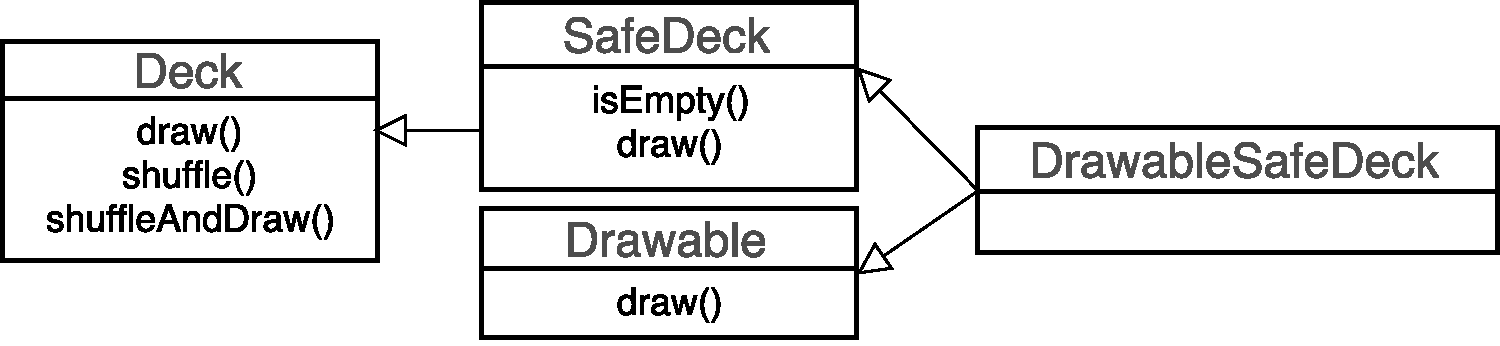
\includegraphics[height=2cm]{pics/DrawableSafeDeck.pdf}
	\caption{UML graph for \lstinline|DrawableSafeDeck|.}\label{fig:drawablesafedeck}
	\saveSpaceFig
\end{figure*}

\vspace{3pt}\begin{lstlisting}
interface DrawableSafeDeck extends Drawable, SafeDeck {}

// main program
DrawableSafeDeck d = new DrawableSafeDeck();
d.shuffleAndDraw(); // ambiguous draw if dynamically dispatched
\end{lstlisting}\vspace{3pt}
From \lstinline|DrawableSafeDeck|'s point of view, the \lstinline|draw| method seems ambiguous. But ideally we would
like \lstinline|shuffleAndDraw| to invoke \lstinline|SafeDeck.draw| because they belong to the same branch. Hence it
seems that we choose dynamic dispatch but also make use of some static type information. Note that this problem can be
solved by the C++ code below:
\vspace{3pt}\begin{lstlisting}
class Deck { public: virtual void draw() {...} ... };
class Drawable {...};
class SafeDeck : public Deck { public: virtual void draw() {...} ... };
class DrawbaleSafeDeck : public Drawable, public SafeDeck {};

// in main
DrawableSafeDeck d;
d.shuffleAndDraw();
\end{lstlisting}\vspace{3pt}
By putting ``\lstinline|virtual|'' in front of every method signature, we are enforcing dynamic dispatch in C++.\\

\noindent\textbf{Our solution:} inspired by that, we propose \textit{hierarchical dispatch} in our model
as the default method lookup algorithm. A \textit{hierarchical invocation}, or \textit{path invocation}, namely
\lstinline|e.I?m()|, is read as
``finding the most specific method \lstinline|m| along the path
\lstinline|I|''. Formally, the meaning of ``along the path \lstinline|I|'' is
that, if the result of hierarchical dispatch finds \lstinline|J.m()| for some \lstinline|J|, then such a \lstinline|J| must be a super type of \lstinline|e|'s dynamic type for sure, and \lstinline|J| must have a subtyping relation with \lstinline|I| (either \lstinline|J <: I| or \lstinline|J >: I|). Intuitively, the most specific \lstinline|m| must be from branch \lstinline|I|, but it can be an updated version after \lstinline|I| because of dynamic dispatch. The formal definition will be introduced later.

On the other hand, \lstinline|e.m()| where \lstinline|e| has static type \lstinline|I|, simply behaves the same as \lstinline|e.I?m()| in our model. Such a dispatching algorithm makes use of both the static type and the dynamic type of the receiver, so it is seemingly a combination of static and dynamic dispatch. Intuitively, the static type specifies one branch to avoid ambiguity, and the dynamic type finds the latest version on that branch. It may still introduce ambiguity when there are multiple paths from the static type to the dynamic type, and those paths cause conflicts. We disallow this kind of conflict to ensure unambiguity. That is to say, we do not allow two methods to override a same base method when they cause conflicts. This is natural, as they are just two versions of the same operation, hence it is no longer an ``unintentional'' conflict, but the diamond problem.

Back to the example, our code below just suffices to meet the expectation:
\vspace{3pt}\begin{lstlisting}
interface Deck {
  void draw() {...}
  void shuffle() {...}
  void shuffleAndDraw() { shuffle(); draw(); }
}
interface Drawable {...}
interface SafeDeck extends Deck {...}
interface DrawableSafeDeck extends Drawable, SafeDeck {}

// main program
new DrawableSafeDeck().shuffleAndDraw() // calls Deck.shuffle, and then SafeDeck.draw
\end{lstlisting}\vspace{3pt}\haoyuan{mention how the language syntax is different from our formalization. FHJ is only a subset.}
Note that the \lstinline|draw()| in \lstinline|shuffleAndDraw()| is short for \lstinline|this.draw()|, and is equivalent to \lstinline|this.Deck?draw()|. It is because the compiler is able to know that the receiver ``\lstinline|this|'' exactly has static type \lstinline|Deck|. Hence hierarchical dispatch eliminates ambiguity in a concise way.\\

\noindent\textbf{Comparison with C++:} as an industrial language, C++ is more practical and flexible to use with lots of features, for example, it handles fields and virtual inheritance, and it allows explicit casts. But the compilation is more or less complicated, and sometimes unclear to programmers, which affects its type safety and people's understanding. The compilation seems to look into the expressions and the real (runtime) types for ambiguity check in method dispatching, and sometimes the errors are thrown by the linker. In contrast, inspired by C++ we formalize the concept of hierarchical dispatch in our model, with type-checking rules and semantics. The compilation only cares about the type of the receiver in method invocation, but the rules ensure type soundness so that the evaluation never throws errors on a program that type-checks. C++ does not hold type soundness for unintentional method conflicts, it actually accepts the diamond inheritance, and only complains on bad invocations. Whereas our model forbids the diamond case, which derives a strong type-safe system, and there are more theoretical aspects in Section~\ref{sec:formalization}. \haoyuan{not sure if this paragraph makes sense or is correct. Needs refs.}


\subsection{Problem 3: Overriding on Individual Branches}\label{subsec:partialoverrides}
We have seen that hierarchical dispatch can dynamically find the latest implementation of a method from one path (or branch). But when
several branches are merged by triangle inheritance, there is usually demand for updating them separately. For example, someone plans to
reuse the other features of \lstinline|DrawableSafeDeck|, but updates the \lstinline|draw| from \lstinline|Drawable| by drawing a rectangle representing deck. Unfortunately in traditional models, the merged branches cannot be separately overridden any longer, since overriding
will hide all branches and break coexistence. Modifying existing code is again unsatisfactory as it affects modularity. The nature way to work around the problem is to define a new component \lstinline|Drawable2| and change the class hierarchy:
\begin{lstlisting}
interface Drawable2 extends Drawable {
  void draw() {
    JFrame frame = new JFrame("Canvas");
    frame.setSize(600, 600);
    frame.getContentPane().setBackground(Color.red);
    frame.getContentPane().add(new Square(10,10,100,100));
    ....
  }
}
interface DrawableSafeDeck extends Drawable2, SafeDeck {}
\end{lstlisting} 
The drawabck of the workaround is obvious: it breaks the existing hierarchy and changes the old code.

\noindent\textbf{Our solution:} an additional feature of our model is \textit{hierarchical overriding}. It allows conflicting methods
to be overridden on individual branches, and hence offers independent extensibility. The above example can be easily realized by:
\vspace{3pt}\begin{lstlisting}
interface DrawableSafeDeck extends Drawable, SafeDeck {
  void draw() override Drawable {
    JFrame frame = new JFrame("Canvas");
    frame.setSize(600, 600);
    frame.getContentPane().setBackground(Color.red);
    frame.getContentPane().add(new Square(10,10,100,100));
    ...
  }
}
// main program, calling draw in DrawableSafeDeck
((Drawable)new DrawableSafeDeck()).draw(); 
\end{lstlisting}\vspace{3pt}

\textbf{Terminology} The \lstinline|draw| methods we saw before this example are called ``original methods'' in this paper, because they are originally defined in its interface.
In contrast, \lstinline|DrawableSafeDeck| defines a ``hierarchical overriding'' method. The difference is that traditional method overriding overrides all branches by defining another original method, whereas hierarchical overriding only refines one branch.

In our model, triangle inheritance allows several original methods (branches) to coexist, and hierarchical dispatch first finds the most specific original method (branch), then it finds the most specific hierarchical overriding on that branch. A quick counter-example is when there are two hierarchical overriding methods on \lstinline|Drawable| in \lstinline|DrawableSafeDeck|, it leads to ambiguity. The compiler is supposed to forbid that during compile time.

A special rule for hierarchical overriding is: it can only refine \textbf{original} methods, and cannot jump over original methods with the same signature. For instance, writing \lstinline|"void draw()| \lstinline|override Deck {...}"| is disallowed in \lstinline|DrawableSafeDeck|, because existing two branches are \lstinline|Drawable.draw| and \lstinline|SafeDeck.draw|, while \lstinline|Deck.draw| is already covered. It does not really make sense to refine an old branch.

% Similar to many OO languages, the model also allows \textit{super method invocation} in a method body. The invocation \lstinline|super.T::m()| will ignore all the subtypes of \lstinline|T|, and only look at \lstinline|T| together with its super interfaces. It should behave the same as \lstinline|new T().m()| in principle.
\section{Formalization}~\label{sec:formalization}
In this section, we present a formal model called \MIM{} (\emph{\textbf{F}eatherweight \textbf{H}ierarchical \textbf{J}ava}), following the similar style of 
Featherweight Java~\cite{Igarashi01FJ}. \MIM{} is a minimal core calculus that formalizes the core concept of hierarchical dispatching and overriding. The syntax, typing rules and small-step semantics are presented.

% \vspace{-2ex}
\subsection{Syntax}
The abstract syntax of \MIM{} interface declarations, method declarations, and expressions is given in Figure~\ref{fig:syntax}. The multiple
inheritance feature of \MIM{} is inspired by Java 8 interfaces, which supports
method implementations via default methods. This feature is 
closely related to \emph{traits}. To demonstrate how
unintentional method conflicts are untangled in \MIM{}, we only focus on a small subset of the interface model. For example, all methods declared
in an interface are either default methods or abstract methods. Default methods provide default implementations for methods. Abstract methods do not
have a method body. Abstract methods can be overridden with future implementations.

\paragraph{Notations}
The metavariables $I, J$ range over interface names; $x$ ranges over variables; $m$ ranges over method names; $e$ ranges over expressions; and $M$ ranges over method declarations. Following Featherweight Java, we assume that the set of variables includes the special variable \kwthis, which cannot be used as the name of an argument to a method. We use the same
conventions as FJ; we write $\overline{I}$ as shorthand for a possibly empty sequence $I_1, ..., I_n$, which may be indexed by $I_i$; and write $\overline{M}$ as shorthand for $M_1 .. M_n$ (with no commas). We also abbreviate operations on pairs of sequences in an obvious way, writing $\overline{I} \; \overline{x}$ for $I_1 \; x_1, ..., I_n \; x_n$, where $n$ is the length of $\overline{I}$ and $\overline{x}$.

\paragraph{Interfaces}
In order to achieve multiple inheritance, an interface can have a set of 
parent interfaces, where such a set can be empty. The interface declaration $\interface{I}{I}{M}$ introduces an interface named $I$ with parent interfaces $\overline{I}$ and a suite of methods $\overline{M}$. The methods of $I$ may either override methods that are already defined in $\overline{I}$ or add new functionality special to $I$, we will illustrate this in more detail later.

\paragraph{Methods}
Original methods and hierarchically overriding methods share the same syntax in our model for simplicity.
The concrete method declaration $\method{I}{m}{I_x}{x}{J}{e}$ introduces a
method named $m$ with result type $I$, parameters $\overline{x}$ of
type $\overline{I_x}$ and the overriding target $J$. The body of the
method simply includes the returned expression $e$. Notably, we have introduced the
\kwoverride{} keyword for two cases: if the overridden interface is exactly the enclosing
interface itself, then such a method is seen as originally defined; otherwise it is a hierarchical overriding method. The definition
of abstract methods is written as $\absmethod{I}{m}{I_x}{x}{J}$, which is
similar to a concrete method but without the method body. 
For simplicity, overloading is not modelled for methods, which
implies that we can uniquely identify a method by its name.

\paragraph{Expressions \& Values}
Expressions can be standard constructs such as variables, method
invocation, object creation, together with cast expressions. 
Object creation is represented by $\new I$\footnote{In Java the corresponding syntax is $\new I\{\}$.}. Fields and primitive types are not modelled in \MIM{}. 
The casts are merely safe upcasts, and in fact, they can be viewed as
annotated expressions, where the annotation indicates its static type.
The coexistence of static and dynamic types is the key to hierarchical dispatch.
A value
``$(I)\new{J}$''
is the final result of multiple reduction steps evaluating an
expression.

For simplicity, \name{} does not formalize statements like assignments and so on because they are orthogonal features to the hierarchical dispatching and overriding feature.
A program in \name{} consists of a list of interface declarations, plus a single expression.

\begin{figure*}[t]
\saveSpaceFig
\begin{displaymath}
\begin{array}{l}
\begin{array}{llrl}
\text{Interfaces}   & IL & \Coloneqq & \interface{I}{I}{M} \\
\text{Methods}      & M  & \Coloneqq & \method{I}{m}{I_x}{x}{J}{e}  \mid
									   \absmethod{I}{m}{I_x}{x}{J} \\
\text{Expressions}  & e  & \Coloneqq & x \mid
e.m(\overline{e}) \mid
\new{I} \mid \; (I)e \\
\text{Context}      & \Gamma & \Coloneqq & \overline{x}:\overline{I} \\
\text{Values}       & v & \Coloneqq & (I) \new{J} \\
%%\\
%%\text{Interface names} & I, J, K & & \\
%%\text{Method names} & m & & \\
%%\text{Variable names} & x & &
\end{array}
\end{array}
\end{displaymath}
\caption{Syntax of \name{}.}\label{fig:syntax}
\saveSpaceFig
\end{figure*}


\begin{figure*}[t]
\saveSpaceFig
\begin{mathpar}
	\framebox{$ I <: J $} \hspace{.5in} \subid \\
	\subtrans \hspace{.5in} \subextends \\
	
	\framebox{$ \judgeewf \Gamma {e:I} $} \hspace{.5in}
	\tvar \\
	\tinvk \\
	% \tpathinvk \\
	% \tsuperinvk \\
	% \tstaticinvk  \\
	\tnew \\
	\tanno \\
	\tmethod \\
	\tabsmethod \\
	\tintf
\end{mathpar}
\saveSpaceFig
\caption{Typing and subtyping of \name{}.}
\label{fig:typingrules}
\end{figure*}

\subsection{Subtyping and Typing Rules}\label{subsec:typingrules}
\paragraph{Subtyping}
The subtyping of \MIM{} consists of only a few rules shown at the top of Figure~\ref{fig:typingrules}.
In short, subtyping relations are built from the inheritance in interface
declarations. Subtyping is both symmetric, reflexive and transitive.

\paragraph{Type-checking}
Details of type-checking rules are displayed at the bottom of Figure~\ref{fig:typingrules}, including expression
typing, well-formedness of methods and interfaces. As a convention, an environment
$\Gamma$ is maintained to store the types of variables, together with
the self-reference $\kwthis$.
% The three rules for method invocation, \textsc{(T-Invk)}, \textsc{(T-PathInvk)} and \textsc{(T-SuperInvk)}
% are very similar, in the sense that they all check the type of the specific method, by using
% an auxiliary function \mtype. \mtype{} is the function for looking up method types, which we will
% illustrate later in Section~\ref{subsec:auxdefs}. After the method
% type is obtained, they all check that the arguments and the receiver
% have compatible types. Additionally, \textsc{(T-PathInvk)} requires the receiver to be the subtype of the specified
% path type, and \textsc{(T-SuperInvk)} checks if the enclosing type directly extends the specified super type.

\textsc{(T-Invk)} is the typing rule for method invocation.
Naturally, the receiver and the arguments are required to be well-typed.
$\mbody$ is our key function for method lookup that implements the
hierarchical dispatching algorithm. The formal definition will be introduced in Section~\ref{sec:auxdefs}.
Here $\mbody(m, I_0, I_0)$ finds the most specific $m$ above $I_0$. ``Above $I_0$'' specifies
the search space, namely the super types of $I_0$ including itself.
For the general case, however, the hierarchical invocation $\mbody(m, I, J)$ finds ``the most specific $m$
above $I$ and along path/branch $J$''. ``Along path $J$'' additionally requires the result to relate to $J$, that is to say,
the most specific interface that has a subtyping relationship with $J$.

In \textsc{(T-Invk)}, as the compilation should not be aware
of the dynamic type, it only requires that invoking $m$ is valid for the static type of the
receiver. The result of $\mbody$ contains the interface that provides the most specific implementation,
the parameters and the return type. We use underscore for the return expression, implying that an empty return expression
from an abstract method is acceptable.
% \textsc{(T-PathInvk)} is the typing judgement for a path invocation. Besides the conditions of \textsc{(T-Invk)}, \textsc{(T-PathInvk)} requires the type of receiver to be the subtype of the specified path type. 
% and \textsc{(T-SuperInvk)} checks if the enclosing type directly extends the specified super type.

\textsc{(T-New)} is the typing rule for object creation $\new{I}$. The
auxiliary function $\canInstantiate(I)$ (see definition in Section~\ref{sec:otherdefs}) checks whether an interface $I$ 
can be instantiated or not. Since triangle inheritance accepts conflicting branches to coexist, the check requires that the most specific method is concrete for each method on each branch.

\textsc{(T-Method)} is more interesting since a method can either be an original method or a hierarchical overriding, though
they share the same syntax and method typing rule. $\mostSpecific(m, I, J)$ is a fundamental function,
used to find ``the most specific interfaces that are above $I$ and
along path $J$, and originally defines $m$'' (see
Section~\ref{sec:auxdefs} for full definition).
By ``most specific interfaces'',
it implies that the inherited super types are excluded. Thus the condition $\mostSpecific(m, I, J) = \{J\}$ indicates a characteristic of a hierarchical overriding: it must override an original method; the overriding is direct and there does not exist any other original method $m$ in between.
Then $\mbody(m, J, J)$ provides the type of the original method, so hierarchical overriding has to preserve the type. Finally the return expression
is type-checked to be subtype of the declared return type. For the definition of an original method, $I$ equals $J$ and the rule is straightforward. \textsc{(T-AbsMethod)} is a similar rule but works on abstract method declarations.

\textsc{(T-Intf)} defines the typing rule on interfaces. The first condition is obvious, namely its methods need to be well checked. The third
condition checks whether the overriding between original methods preserves typing. In this condition we again use some helper functions defined in  Section~\ref{sec:auxdefs}. $I[m\ \kwoverride\ I]$ is defined if $I$ originally defines $m$, and $\canOverride(m, I, J)$ checks whether $I.m$ has the same type as $J.m$. Generally the preservation of method type is required for any super type $J$ and any method $m$.

The second condition of \textsc{(T-Intf)} is more complex and is the key to type soundness. Unlike C++ which rejects on ambiguous calls,
\MIM{} rejects on the definition of interfaces when they form a diamond. Consider the case when the second condition is broken: $\mbody(m, J, J)$
is defined but $\mbody(m, I, J)$ is undefined for some $J$ and $m$. This indicates that $m$ is available and unambiguous from the perspective of $J$,
but is ambiguous to $I$ on branch $J$. It means that there are multiple overriding paths of $m$ from $J$ to $I$, which forms a diamond. Hence rejecting
that case meets our expectation. Below is an example (Figure~\ref{fig:examplesmbody} (e)) that illustrates the reason why this condition is needed:
%\bruno{what is the purpose of this example:
%  state-it upfront please. Is this example meant to ilustrate T-Inf?
%  Then it's better to have the example together with the text
%  explaining T-inf.} \yanlin{revised.please check whether you're happy with it.}
\begin{lstlisting}
interface T                 { T m() override T { return new T(); } }
interface A extends T       { T m() override T { return new A(); } }
interface B extends T       { T m() override T { return new B(); } }
interface C extends A, B {}
((T) new C()).m()
\end{lstlisting}
This program does not compile on interface $C$, because of the second condition in \textsc{(T-Intf)}, where $I$ equals $C$ and $J$ equals $T$.
By the algorithm, $\mbody(m, T, T)$ will refer to $T.m$, but $\mbody(m, C, T)$ is undefined, since both $A.m$ and $B.m$ are most specific
to $C$ along path $T$, which forms a diamond. The expression \lstinline|((A) new D()).m()| is one example of triggering ambiguity, but \MIM{}
simply rejects the definition of $C$. To resolve the issue, the programmer need to have an overriding method in $C$, to explicitly merge
the conflicting ones.

Finally, rule \textsc{(T-Anno)} is the typing rule for a cast expression. By the rule, only upcasts are valid.

\subsection{Small-step Semantics and Congruence}
Figure~\ref{fig:smallstep} defines the small-step semantics and
congruence rules of \MIM{}. When evaluating an expression, they
are invoked and produce a single value in
the end. %\haoyuan{we need to be consistent on paragraph upper/lower case.}

\paragraph{Semantic Rules} \textsc{(S-Invk)} is the only computation rule we need for method invocation.
As a small-step rule and by congruence, it assumes that the receiver and the arguments are already values.
Specifically, the receiver $(J)\new{I}$ indicates the dynamic type $I$
together with the static type $J$. Therefore $\mbody(m, I, J)$ carries out hierarchical dispatching, acquires
the types, the return expression $e_0$ and the interface $I_0$ which provides the most specific method.
Here we use $e_0$ to imply that the return expression is forced to be non-empty because it requires a concrete implementation. Now the
rule reduces method invocation to $e_0$ with substitution.
Parameters are substituted with arguments, and the \lstinline|this| reference is substituted by the receiver,
and in the meanwhile the static types are recorded via annotations. Finally the return type $I_e$ is put in the front as an annotation.
\paragraph{Congruence Rules} \textsc{(C-Receiver)}, \textsc{(C-Args)} and \textsc{(C-FReduce)} are natural congruence rules
on receivers, arguments, and cast-expressions, respectively. \textsc{(C-StaticType)} automatically adds an annotation $I$ to the new
object $\new{I}$. \textsc{(C-AnnoReduce)} merges nested upcasts into a single upcast with the outermost type.



\begin{comment}
\paragraph{Example} In contrast with the counter-example in Section~\ref{subsec:typingrules}, it is better to understand semantics by
well-compiled examples. Here we abstract a variant of the \lstinline|DrawableDeck| example:

\vspace{3pt}\begin{lstlisting}
interface Void       {}
interface JFrame     {}
interface Deck       { Void draw() override Deck { return new Void(); } }
interface Drawable { JFrame draw() override Drawable; }
interface DrawableDeck extends Drawable, Deck {
  JFrame draw() override Drawable {
    return new JFrame();
  }
}

((Drawable) new DrawableDeck()).draw()
\end{lstlisting}\vspace{3pt}
We put \lstinline|Drawable.draw| as an abstract method instead, but hierarchically override it in \lstinline|DrawableDeck|.
By typing rules, the code is well-compiled. And during runtime,
\begin{align*}
	& ((Drawable) new DrawableDeck()).draw() \\
\rightarrow & (JFrame) new JFrame()
\end{align*}
\end{comment}
% \section{Method Lookup Algorithm and Auxiliary Definitions}\label{sec:auxdefs}
\section{Key Algorithms and Type-Soundness}\label{sec:auxdefs}
In this section, we present the fundamental algorithms and auxiliary
definitions used in our formalization, and show that the resulting
calculus is type sound. The functions presented in this section are
the key components that implement our algorithm for method lookup.

\subsection{Method Lookup Algorithm in \mbody{}}\label{subsec:mbodydef}

$\mbody(m, I_d, I_s)$ denotes the method body lookup function.
We use $I_d, I_s$, since $\mbody$ is usually invoked by a receiver of a method $m$, with its dynamic type $I_d$ and static type $I_s$. Such a function returns the most specific method implementation. More
accurately, $\mbody$ returns the parameters, returned expression
(empty for abstract methods) and the types for the method. It considers both originally-defined methods and hierarchical overriding methods, so $\mostSpecific$ and $\mostSpecificOverride$ (see the definition in Section~\ref{sec:mostSpecific} and Section~\ref{sec:mostSpecificOverride}) are both invoked.
 The formal definition gives the expected results
for the earlier examples in Figure~\ref{fig:examplesmbody}.

\begin{flalign*}
	& \rhd \textit{Definition of } \mbody(m, I_d, I_s): & \\
	& \bullet \mbody(m, I_d, I_s) = (J, \overline{I_x} \; \overline{x}, I_e \; e_0) & \\
	& \indent\indent \textrm{with: } \mostSpecific(m, I_d, I_s) = \{I\} & \\
	& \hspace{.77in} \mostSpecificOverride(m, I_d, I) = \{J\} & \\
	& \hspace{.77in} J[m\ \kwoverride\ I] = \method{I_e}{m}{I_x}{x}{I}{e_0} & \\
	& \bullet \mbody(m, I_d, I_s) = (J, \overline{I_x} \; \overline{x}, I_e \; \o) & \\
	& \indent\indent \textrm{with: } \mostSpecific(m, I_d, I_s) = \{I\} & \\
	& \hspace{.77in} \mostSpecificOverride(m, I_d, I) = \{J\} & \\
	& \hspace{.77in} J[m\ \kwoverride\ I] = \absmethod{I_e}{m}{I_x}{x}{I} & \\
\end{flalign*}
To calculate $\mbody(m, I_d, I_s)$, the invocation of $\mostSpecific$ looks for the most specific original methods and their interfaces, and expects a singleton set, so as to avoid unambiguity. Furthermore, the invocation of $\mostSpecificOverride$ also expects a unique (unambiguous) most specific hierarchical override. And finally the target method is returned.

\subsection{Finding the Most Specific Origin: \mostSpecific}\label{sec:mostSpecific}
\haoyuan{Visualize findorigin and findoverride with some figures.}
We proceed to give the definitions of two core functions that support method lookup, namely \mostSpecific{} and \mostSpecificOverride. Generally,
$\mostSpecific(m, I, J)$ finds the set of most specific interfaces where $m$ is originally defined, they should be above $I$ and
along path $J$. ``Along path $J$'' means one should be either a subtype or a super type of $J$. Finally with $\prune$ (defined in Section~\ref{sec:otherdefs})
the overridden interfaces will be filtered out.

\begin{flalign*}
	& \rhd \textit{Definition of } \mostSpecific(m, I, J): & \\
	& \bullet \mostSpecific(m, I, J) = \prune(origins) & \\
	& \indent\indent \textrm{with: } origins = \{K \mid \subt{I}{K}, \textrm{ and } \subt{K}{J} \; \lor \; \subt{J}{K}, &\\
	& \hspace{1.62in} \textrm{ and } K[m\ \kwoverride\ K] \textrm{ is defined} \} &
\end{flalign*}
By the definition, an interface belongs to $\mostSpecific(m, I, J)$ if and only if:
\begin{itemize}
	\item It originally defines $m$;
	\item It is a super type of $I$;
	\item It is either a super type or a subtype of $J$ (including $J$ itself);
	\item Any subtype of it does not belong to the same result set because of $\prune$.
\end{itemize}

\subsection{Finding the Most Specific Overriding: \mostSpecificOverride}\label{sec:mostSpecificOverride}
The $\mostSpecific$ function only focuses on original method
implementations, all the hierarchical overriding methods are omitted
during that step. On the other hand, $\mostSpecificOverride(m, I, J)$
has the assumption that $J$ defines an original $m$, and this function
tries to find the interfaces with the most specific implementations that hierarchically overrides such an $m$. Formally,

\begin{flalign*}
	& \rhd \textit{Definition of } \mostSpecificOverride(m, I, J): & \\
	& \bullet \mostSpecificOverride(m, I, J) = \prune(overrides) & \\
	& \indent\indent \textrm{with: } overrides = \{K \mid \subt{I}{K}, \; \subt{K}{J} \textrm{ and } K[m\ \kwoverride\ J] \textrm{ is defined} &
\end{flalign*}
By the definition, an interface belongs to $\mostSpecific(m, I, J)$ if and only if:
\begin{itemize}
	\item It is between $I$ and $J$;
	\item It hierarchically overrides $J.m$;
	\item Any subtype of it does not belong to the same set.
\end{itemize}


\subsection{Other Auxiliaries}\label{sec:otherdefs}
Below we give other minor definitions of the auxiliary functions that are used in previous sections.

%%%%============================ I[m override J] ================%%%%%%%%
\begin{flalign*}
	& \rhd \textit{Definition of } I[m\ \kwoverride\ J]: & \\
	& \bullet I[m\ \kwoverride\ J] = \method{I_e}{m}{I_x}{x}{J}{e_0} & \\
	& \indent\indent \textrm{with: }
	  \kwinterface \; I \; \kwextends \; \overline{I} \; \{ \method{I_e}{m}{I_x}{x}{J}{e_0} \ldots \} & \\
	& \bullet I[m\ \kwoverride\ J] = \absmethod{I_e}{m}{I_x}{x}{J} & \\
	& \indent\indent \textrm{with: }
	\kwinterface \; I \; \kwextends \; \overline{I} \; \{ \absmethod{I_e}{m}{I_x}{x}{J} \ldots \} & \\
\end{flalign*}
Here $I[m\ \kwoverride\ J]$ is basically a direct lookup for method $m$ in the body of $I$, where such a method
overrides $J$ (like static dispatch). The method can be either concrete or abstract, and the body of definition is returned. Notice that
by our syntax, $I[m\ \kwoverride\ I]$ is looking for the originally-defined method $m$ in $I$.
%%%%============================ I[m override J] end================%%%%%%%%

%%%%============================ prune(set) ================%%%%%%%%
\begin{flalign*}
	& \rhd \textit{Definition of } \prune(set): & \\
	& \bullet \prune(set) = \{I \in set \; | \; \nexists J \in set\setminus I, J <: I\} &
\end{flalign*}
The $\prune$ function takes a set of
types, and filters out those that have subtypes in the same set. In the returned set,
none of them has subtyping relation to one another, since all super types have been removed.
%%%%============================ prune(set) end ================%%%%%%%%

%%%%============================ canOverride ================%%%%%%%%
\begin{flalign*}
	& \rhd \textit{Definition of } \canOverride(m, I, J): & \\
	& \bullet \canOverride(m, I, J) = True & \\
	& \indent\indent \textrm{with: } I[m\ \kwoverride\ I] = I_e \; m(\overline{I_x} \; \overline{x}) \; \kwoverride \; I \ldots & \\
	& \hspace{.77in} J[m\ \kwoverride\ J] = I_e \; m(\overline{I_x} \; \overline{y}) \; \kwoverride \; J \ldots &
\end{flalign*}
$\canOverride$ just checks that two original $m$ in $I$ and $J$ have the same type.
%%%%============================ canOverride end ================%%%%%%%%

%%%%============================ canInstantiate ================%%%%%%%%
\begin{flalign*}
	& \rhd \textit{Definition of } \canInstantiate(I): & \\
	& \bullet \canInstantiate(I) = True & \\
	& \indent\indent \textrm{with: } \forall m, \forall J \in \mostSpecific(m, I, I), \mostSpecificOverride(m, I, J) = \{K\}, & \\
	& \hspace{.77in} \textrm{ and } K[m\ \kwoverride\ J] = \method{I_e}{m}{I_x}{x}{J}{e_0} &
\end{flalign*}
$\canInstantiate(I)$ checks whether interface $I$ can be instantiated by the keyword $\kwnew$.
$\mostSpecific(m, I, I)$ represents the set of branches $I$ inherits on method $m$. $I$ can be instantiated
if and only if for every branch, the most specific implementation is unambiguous and non-abstract.
%%%%============================ canInstantiate end ================%%%%%%%%

\subsection{Properties}

We present the type soundness of the model by a few theorems below, following the standard technique of
subject reduction and progress proposed by Wright and Felleisen~\cite{Wright1994}. The proof, together with some lemmas, are
in Appendix. Type soundness states that if an expression is well-typed, then after many reduction
steps it must reduce to a value, and its annotation is the same as the static type of the original expression.

\begin{theorem}[Subject Reduction]~\label{theorem_subject}
If $\judgeewf \Gamma {e : I}$ and $e \rightarrow e'$, 
then $\judgeewf \Gamma {e' : I}$.
\end{theorem}
\begin{proof}
See Appendix~\ref{appendix_proof}.
\end{proof}

\begin{theorem}[Progress]~\label{theorem_progress}
Suppose $e$ is a well-typed expression, if $e$ includes 
$\left((J)\emph{\kwnew}\;I()\right).m(\overline{v})$ as a sub-expression, then $\mbody(m, I, J) = (I_0, \overline{I_x} \; \overline{x}, I_e\; e_0)$ and $\num{\overline{x}} = \num{\overline{v}}$ for some $I_0$, $\overline{I_x}$, $\overline{x}$, $I_e$ and $e_0$.
\end{theorem}
\begin{proof}
See Appendix~\ref{appendix_proof}.
\end{proof}

\begin{theorem}[Type Soundness]~\label{theorem_soundness}
If $\judgeewf \o {e : I}$ and $e \to^* e'$ with $e'$ a normal form, then $e'$ is 
a value $v$ with $\judgeewf \o {v:I}$.
\end{theorem}
\begin{proof}
Immediate from Theorem~\ref{theorem_subject} and Theorem~\ref{theorem_progress}.
\end{proof}
Note that in Theorem~\ref{theorem_progress}, ``$\#(\overline{x})$'' denotes the length of
$\overline{x}$.

Our theorems are stricter than those of Featherweight Java~\cite{Igarashi01FJ}. Specifically, in both term substitution (a lemma in Appendix)
and subject reduction, reduction may lead to a term with a subtype in
FJ, but in \MIM{} types are unchanged. The difference is due to
%%subtyping; the parameter or \lstinline|this| reference requires some type $I$, but a value with a more specific type,
%%which is subtype of $I$, can be passed. However, as 
the fact that \MIM{} keeps track of the static types during
reduction. 
In FJ, the information about the static types is lost. 

%the annotations in the
%substitution actually ensures the type to be unchanged.
\section{Discussion}\label{sec:discussion}
In this section, we will discuss the design space and reflect about some of the design decisions of our work. We relate 
our language to traits, Java interfaces as well as other languages. Furthermore we discuss
ways to improve our  work.\bruno{references please!!!} \haoyuan{Done}

\subsection{Abstract Methods}

Abstract methods are one of the key features in most general OO languages. For example, Java interfaces were designed
to include only method declarations, and those abstract methods can be implemented in a class body. 
The formal Featherweight Java model~\cite{Igarashi01FJ} does not include abstract methods because of its orthogonality
to the core calculus. In traits the
similar idea is to use keywords like ``\textbf{require}'' for abstract method declarations~\cite{scharli03traits}.
Abstract methods provide a way to
delay the implementations to future subtypes. Using overriding, they also help to ``exclude'' existing implementations.

In our formalized calculus, however, abstract methods are not a completely orthogonal feature. The $\canInstantiate$ function
has to check whether an interface can be instantiated, by looking at all the inherited branches and seeing if each most specific method
is abstract or not.

Our formalization has a simple form of abstract methods, which behave similarly to conventional methods with respect to conflicts.
Other languages support more complicated behaviour.
For instance, in Java 8 when putting two identical abstract methods together by multiple inheritance, there is no conflict error. We omit
that case for two reasons. First, our formalization just treats abstract methods as concrete methods with an empty body, and that simplifies
the rules and the proof a lot. Second, our design choice tends to give more sense on those interesting cases, just as we reject the simple case of diamond inheritance. The triangle inheritance should distinguish and treat differently on the two methods instead of fusing them, since they represent different operations, even if they are abstract. Thus our model adopts a very conservative behaviour rather than automatically merging 
methods, and implicitly assumming diamond inheritance.

\subsection{Orthogonal \& Non-Orthogonal Extensions}\label{sec:orthoext}

Our model is designed as a minimal calculus for focusing only on resolving unintentional conflicts. Therefore, we have omitted a number of
common orthogonal features including primitive types, assignments, method overloading, covariant method return types, static dispatch, and so on.
Those features can be modularly added to the model without breaking type soundness \haoyuan{correct?}. For example, we present the additional syntax, typing and semantic rules of static invocation below as an extension:

\begin{mathpar}
	\begin{array}{llrl}
		\text{Expressions}  & e  & \Coloneqq & \ldots \; \mid \; e.J_0@J_1::m(\overline{e})
	\end{array} \\
	\tstaticinvk \\
	\sstaticinvk
\end{mathpar}
A static invocation $e.J_0@J_1::m(\overline{e})$ aims at finding the method $m$ in $J_0$ that hierarchically overrides $J_1$, thus $J_0[m\ \kwoverride\ J_1]$ is invoked. As shown in \textsc{(S-StaticInvk)}, static dispatch needs a receiver to involve in the substitution for ``$\kwthis$'' reference, so as to provide the latest implementations. In fact, static dispatch is common in OO programming, as it provides a shortcut to the reuse of old implementation easily, and super calls can also rely on this feature. For convenience we just make it simple above, whereas in languages like C++ or Java, the static or super invocations are more flexible hence complicated; they can climb the class hierarchy. 

One typical non-orthogonal extension to \MIM{} could be to have fields.
The design of \MIM{} can be viewed as an extension to Java 8 with default methods which allows for unintentional method conflicts.
Like Java interfaces and traits, state is forbidden in \MIM{} since having state in OO multiple inheritance is a non-trivial issue. There has been some related work on it, such as C++ that uses virtual inheritance~\cite{ellis1990annotated}. In our model, however, we can perhaps borrow the idea of \textit{interface-based programming}~\cite{classless}, which models state with abstract state operations. This can be realized by extending our current model with static methods and anonymous classes from Java. To directly support fields it requires more discussions and experiments, we leave them as our future work.

\subsection{Loosening the Model}

For the goal of simplifying the model and type soundness proof, we have added a few constraints in the minimal calculus. Our language simply rejects the diamond inheritance, see the example below:

\vspace{3pt}\begin{lstlisting}
interface A { void m() {...} }
interface B extends A { void m() {...} }
interface C extends A { void m() {...} }
interface D extends B, C {}
\end{lstlisting}\vspace{3pt}
In the example, both $B.m$ and $C.m$ override $A.m$, so we think they should represent the same operation. In that case, we believe that D inherits
both conflicting methods without an explicit override, and it is in fact an intention conflict. Our calculus rejects these intentional conflicts by rule \textsc{(T-Intf)}, where $D$ is considered to be ill-formed. Nonetheless, as a general-purpose language, C++ accepts the definition of $D$, but forbids a cast from $D$ to $A$ because of ambiguity. For the conciseness of the proof, our language is more conservative on interfaces, but open on up-casts. We could also loosen the model and perform ambiguity check on casts and other expressions. We need to handle more cases than C++, for instance, in the above program assume that $B.m$ and $C.m$ are hierarchical overrides on $A$, it is still a diamond.

Another case is about the restriction on hierarchical overrides. In our language model there are two types of methods (though they share the same syntax): original methods and hierarchical overrides. We require that a hierarchical override should only override an original method. Yet from the idea of encapsulation and modularity on programs, we could also allow an override to work on another override, which forms a series of overrides.

\haoyuan{more. 1) Path Invocation, more generalized diamond inheritance: not clear; other method resolution techniques: no example; better code reuse with other kinds of method invocation: no example. }

\section{Related Work}~\label{sec:relatedwork}
We describe related work in four parts. We first discuss mainstream popular multiple 
inheritance models and the specific models (C++ and \csharp) which are closest to our work. Then we 
discuss related techniques used in \self. Finally, we discuss the foundation and related work of our formalization.

\subsection{Mainstream Multiple Inheritance Models}
Multiple inheritance is a useful feature in object-oriented
programming, although it is difficult to model and can 
cause various problems (e.g. the diamond problem~\cite{Sak89dis,Singh1995}).  
There are many existing languages/models that support multiple 
inheritance~\cite{ellis1990annotated,scala-overview,bracha90mixin,scharli03traits,malayeri2009cz,csharpdoc,Moon1986,Flatt1998,Ancona2003}. 
The mixin models~\cite{bracha90mixin,Flatt1998,van1996encapsulation,Ancona2003,Hendler86} allow naming components 
that can be applied to various classes as reusable functionality units. However, the linearization (total ordering) of mixin 
inheritance cannot provide a satisfactory resolution in some cases and restricts the flexibility of mixin composition. 
Scala traits~\cite{scala-overview} are in fact linearized mixins and hence have the same problem as mixins.

Simplifying the mixins approach, traits~\cite{scharli03traits,Ducasse:2006:TMF:1119479.1119483} draw a
strong line between units of reuse and object factories. Traits act
as units of reuse, containing functionality code. Classes, on the
other hand, are
assembled from traits and act as object factories. Java 8
interfaces are closely related to traits: concrete method
implementations are allowed (via the \textbf{\texttt{default}}
keyword) inside interfaces, thus allowing for a restricted form 
of multiple inheritance.
There are also proposals such as FeatherTrait Java~\cite{Liquori08ftj} 
for extending Java with traits. Extensions~\cite{reppy2006foundation,Reppy:2007:MT:2394758.2394784} to 
the original trait model exists with various advanced features, such as \emph{renaming}. As discussed in Section~\ref{sec:overview},
the renaming feature gives a workaround to the unintentional method conflicts
problem. However, it breaks structural subtyping.

\begin{comment}
There are also proposals for extending Java with traits. For example, 
FeatherTrait Java (FTJ) [14] extends FJ [13] with statically-typed traits, 
adding trait-based inheritance in Java. Except for few, mostly syntac- tic details, 
their work can be emulated with Java 8 interfaces. There are also extensions 
to the original trait model, with operations (e.g. renaming [18], which breaks 
structural sub- typing) that default methods and interfaces cannot model.
\end{comment}

Malayeri and Aldrich proposed a model CZ~\cite{malayeri2009cz} which
aims to do multiple inheritance without the diamond problem.
Inheritance is divided into two concepts: inheritance dependency and
implementation inheritance.  Using a combination of
\textbf{\texttt{requires}} and \textbf{\texttt{extends}}, a program
with diamond inheritance is transformed to one without
diamonds. Moreover, fields and multiple inheritance can coexist.
However untangling inheritance also untangles the class structure. In
CZ, not only the number of classes but also the class hierarchy
complexity increases.

The above-mentioned models/languages support multiple inheritance, 
focusing on diamond inheritance.
They handle method conflicts in the same way, by simply disallowing
two methods with the same signature from two different units to
coexist. In contrast, our work provides mechanisms that allow 
methods with the same signatures, but different parents to coexist 
in a class. Disambiguation is possible in many cases by using both 
static and dynamic type information during method dispatching.
In the cases where real ambiguity exists, \MIM{}'s type system can
reject interface definitions and/or method calls statically.

\subsection{Resolving Unintentional Method Conflicts}\label{subsec:middleman}
A few language implementations have realized the problem of
unintentional conflicts and provide some support for it.

\begin{comment} %C++ related work with code explaination
\noindent {\bf C++ model.}
C++ supports a very flexible inheritance model and allows programmers to choose either static dispatch or dynamic dispatch for method lookup.
It allows unintentional conflicts and uses static dispatch to resolve them, as discussed in Section~\ref{sec:overview}. For example, given the following code
\begin{lstlisting}[language=Java]
class A { public: void m() {cout << "MA" << endl;} };
class B { public: void m() {cout << "MB" << endl;} };
class C : public A, public B { 
	void m() {cout << "MC" << endl;}
};
void func(A* a) { a->m(); }
int main() {
	C* c = new C();
	c->B::m();
	func(c); 
	return 0; //Running result: MB MA
}
\end{lstlisting}
The running result is $MB \; MA$, meaning that it uses static dispatch (looks at the static types) for method \lstinline|m()|. 
On calling \texttt{func(c)}, in spite that the dynamic type of \texttt{c} is class \texttt{C}, the method call still dispatches to 
\lstinline|A.m|.
However, we can alter the code a little bit with \textbf{\texttt{virtual}} methods and the result will be totally different:
\begin{lstlisting}[language=c++]
class A { public: virtual void m() {cout << "MA" << endl;} };
class B { public: virtual void m() {cout << "MB" << endl;} };
class C : public A, public B { 
    public: virtual void m() {cout << "MC" << endl;}
};
void func(A* a) { a->m(); }
int main() {
	C* c = new C();
	c->B::m();
	func(c); 
	return 0; //Running result: MB MC
}
\end{lstlisting}
Now the running result will be $MB \; MC$. With virtual methods, dynamic dispatch is used and 
method lookup algorithm will find the most specific method definition of $m$, namely \lstinline|C.m| at this time.
Although C++ support this flexibility, dynamic dispatching on
unintentional conflicting methods is problematic, as discussed in
Section~\ref{sec:overview}.\bruno{where in the overview are we
  discussing this?}
Furthermore, compared to our
model, C++ does not support hierarchical overriding.
\end{comment}

\noindent {\bf C++ model.}
C++ supports a very flexible inheritance model.
C++ allows the existence of unintentional conflicts and users may specify a hierarchical path via casts for disambiguation, as discussed in Section~\ref{sec:overview}. 
With virtual methods, dynamic dispatch is used and 
method lookup algorithm will find the most specific method definition. 
A contribution of our work is to provide a minimal formal model of
hierarchical dispatching, whereas C++ can be viewed as a real-world
implementation. There are several
formalizations~\cite{Wasserrab2006,ramananandro2012mechanized,Ramalingam1997}
in the literature modeling various C++ features. However, as far as we know, there is no formal model that
captures this aspect of the C++ method dispatching model. Apart from this, as discussed in Section~\ref{subsec:loosen}, \name{} conservatively rejects some interface/class definitions that C++ accepts, and upcasts are never rejected since they are used for ambiguity resolution.
\bruno{The discussion points out further differences. We need to refer
to that discussion here too.}\yanlin{added.}

Although C++ supports hierarchical dispatching, it does not support
hierarchical overriding.  However, there is a possible
workaround\footnote{https://stackoverflow.com/questions/44632250/can-i-do-mimic-things-likes-this-partial-override-in-c} that mimicks hierarchical
overriding.  We call it the \emph{MiddleMan} approach, as shown in
Figure~\ref{fig:middleman}. In this example, classes \texttt{A} and
\texttt{B} are two classes that both define a method with the same
name \texttt{m}
unintentionally.

Class \texttt{MiddleMan}, as its name suggests, acts as a middle man between its class \texttt{C} and its parents \texttt{A, B}. \texttt{MiddleMan} defines a virtual method \texttt{m} that overrides a parent method \texttt{m} and delegates the implementation to another method \texttt{m\_impl} that takes $\kwthis$ as parameter. C++ supports method overloading, so that multiple \texttt{m\_impl} methods with different parameter types can coexist. When defining class \texttt{C}, we specify the parents to be \texttt{MiddleMan<A>, MiddleMan<B>} instead of \texttt{A, B}. In this way, programmers may define new versions of \texttt{A.m} and \texttt{B.m} in class \texttt{C} by providing the corresponding \texttt{m\_impl} methods. Then in the client code, the method call \texttt{((A*)c)->m()} will print out string \texttt{"MA2"}, as expected. Although this workaround can help us defining partial method overrides to a certain extent, the drawbacks are obvious. Firstly, the approach is complex and requires the pre-knowledge of the programmer to this approach. Moreover, the lack of direct syntax support makes MiddleMan code cumbersome to write. Finally, the approach is ad-hoc, meaning that the class \texttt{MiddleMan} shown in Figure~\ref{fig:middleman} is not general enough to be used in other cases: more middle-mans are needed if partial method overrides happens in other classes; and it is even worse when return types differ.

\begin{figure*}[t]
\begin{lstlisting}
class A { public: virtual void m() {cout << "MA" << endl;}};
class B { public: virtual void m() {cout << "MB" << endl;}};
template<class C>
class MiddleMan : public C {
    void m() override final { m_impl(this); }
  protected:
    virtual void m_impl(MiddleMan*) { return this->C::m(); }
};
class C : public MiddleMan<A>, public MiddleMan<B> { 
private:
    void m_impl (MiddleMan<A>*) override {cout << "MA2" << endl;}
    void m_impl (MiddleMan<B>*) override {cout << "MB2" << endl;}
};
int main()
{
    C* c = new C();
    ((A*)c)->m();         //print "MA2"
    return 0;
}
\end{lstlisting}
\caption{The \emph{MiddleMan} approach.}
\label{fig:middleman}
\end{figure*}

\noindent  {\bf \csharp{} Explicit method implementations.}
Explicit method implementations is a special feature supported by
\csharp{}. As described in \csharp{} documentation~\cite{csharpdoc}, a
class that implements an interface can explicitly implement a member
of that interface. When a member is explicitly implemented, it can
only be accessed through an instance of the interface. Explicit
interface implementations allow an interface to inherit multiple 
interfaces that share the same member names and give each interface
member a separate implementation. 

Explicit interface member implementations have two advantages.
Firstly, they allow interface implementations to be excluded 
from the public interface of a class. This is particularly useful when a class implements an internal 
interface that is of no interest to a consumer of that class or struct.
Secondly, they allow disambiguation of interface members with the 
same signature. However, there are two critical differences to \MIM{}:
(1) default method implementations are not allowed in \csharp{} interfaces; 
(2) there is only one level of conflicting method implementations at the
class that implements the multiple parent interfaces. Further
overriding of those methods is not possible in subclasses.

\subsection{Hierarchical Dispatch in \self{}}
As we have discussed before, although the mix of static and dynamic dispatch is 
particularly useful under certain circumstances, it has received little research attention. 
In the prototype-based language \self{}~\cite{Chambers1991}, inheritance is a basic feature.
\self{} does not include classes but instead allows individual objects to inherit from (or delegate to) other objects. 
Although it is different from class-based languages, the multiple inheritance model is somehow similar. The \self{}
language supports multiple (object) inheritance in a clever way. It not only develops the new inheritance
relation with \emph{prioritized parents} but also adopts \emph{sender path tiebreaker rule} for method lookup.
In \self{} ``\emph{if two slots with the same name are defined in equal-priority parents of the receiver, but only 
one of the parents is an ancestor or descendant of the object containing the method that is sending the message,
then that parent's slot takes precedence over the over parent's slot}''. 
Similarly to our model, this sender path tiebreaker rule resolves ambiguities between unrelated slots. However,
it is used in a prototype-based language setting and it does not support method hierarchical overriding as \MIM{} does.

\subsection{Formalization Based on Featherweight Java}
Featherweight Java (FJ)~\cite{Igarashi01FJ} is a minimal core calculus of the Java language, 
proposed by Igarashi et. al. There are many models built on Featherweight Java, 
including FeatherTrait~\cite{Liquori08ftj}, Featherweight defenders~\cite{goetz12fdefenders}, Jx~\cite{Nystrom2004}, 
Featherweight Scala~\cite{Cremet2006}, and so on.
FJ provides the standard model of formalizing Java-like object-oriented languages and 
is easily extensible. In terms of formalization, the key novelty of our model is making use of various types (such as parameter types, method return types, etc) as upcasts along with various terms. As far as we know, this technique has not appeared in the literature before. This notion is of vital importance in our hierarchical dispatch algorithm, and it allows for a
more precise subject-reduction theorem as discussed in
Section~\ref{sec:formalization}.










\section{Conclusion}


This paper proposes \MIM{} as a formalized multiple inheritance model for
unintentional method conflicts. Previous approaches 
either do not support unintentional method conflicts, thus have to
compromise between code reuse and type safety, or do not fully support
overriding in the presence of unintentional conflicts. To deal with unintentional method conflicts we
introduce two key mechanisms: hierarchical dispatching and
hierarchical overriding. Hierarchical dispatching is inspired by the
mechanisms in C++. We provide a minimal formal model of hierarchical
dispatching in \MIM{}. Such an algorithm makes use of both dynamic type
information and static information from either upcasts or parameters'
information. It not only offers great code reuse like
dynamic dispatch but also ensures unambiguity by our algorithm for
method resolution. Additionally we introduce \emph{hierarchical
  overriding} to allow conflicting methods in different branches to be
individually overridden.

\MIM{} is formalized following the style of
Featherweight Java and proved to be sound. A prototype interpreter is
implemented in Scala. We believe that the formalization of
hierarchical dispatching features is general and
can be safely embedded in other OO models, so as to have support for the \wordfork{}
inheritance.

Our model can certainly be improved in some aspects. 
As discussed in Section~\ref{sec:discussion}, there are orthogonal and
non-orthogonal features that can potentially be added to the design space. 
The future work relates to loosening the model without giving up its soundness,
together with more exploration on supporting fields in the multiple inheritance setting.


%%
%% Bibliography
%%

%% Please use bibtex, 

\bibliography{paper}
\appendix
\section{Appendix}

\subsection{Proofs}~\label{appendix_proof}
\begin{lemma}~\label{lemma0}
% $\textit{If } \mtype(m, I, J) = \overline{D} \rightarrow D, \textit{ and } \mbody(m, I, J) = \overline{x}.e, 
%  \textit{ then for some } J_0 \textit{ with } I <: J_0, \  \exists C <: D, \textit{ such that }  
%  \judgeewf {\overline{x}:\overline{D}, \kwthis:J_0} {e:C} $.
$\textit{If } \mbody(m, I, J) = (J', \overline{I_X} \; \overline{x}, I_E \; e), 
 \textit{ then for some } J_0 \textit{ with } I <: J_0, \  \exists I' <: I_E, \textit{ such that }  
 \judgeewf {\overline{x}:\overline{I_X}, \kwthis:J_0} {e : I'} $.
\end{lemma}

 \begin{proof}~\\
 $\textit{The base case: if } m \textit{ is defined in } I, \textit{ then it is easy since } m 
 \textit{ is defined in } I \textit{ and } 
 \judgeewf {\overline{x}:\overline{I_X}, \kwthis : I} {e : I_E} \textit{ by (T-METHOD)}.
 \textit{ The induction step is also straightforward. }
 $
 \end{proof}


\begin{lemma}[Method Type Preservation]~\label{lemma2}
$\textit{If } \mtype(m, I) = \overline{I_X} \rightarrow I_E, \textit{ then } \mtype(m, J) = \overline{I_X} \rightarrow I_E 
\textit{ for all } J \subtype I.
$
\begin{proof}~\\
Straight induction on the derivation of $J \subtype I$. Whether $m$ is defined in $J$ or not, $\mtype(m, J)$ should 
be the same as $\mtype(m, K)$ where $J \; \kwextends \; K \{...\}$.
\end{proof}
\end{lemma}


%%%%%%%%%%%%%%%%%%%%%%%%%%%%%%%%%%%%%%%%%%%%%%%%%%%%
\begin{lemma}[Term Substitution Preserves Typing]~\label{lemma1}
$\textit{If } \ \judgeewf {\Gamma, \ \overline{x}:\overline{I_X}} { e : I } \textit{ , and }
\judgeewf {\Gamma} {\overline{y}:\overline{I_Y}} \textit{ where } \overline{I_Y} \subtype \overline{I_X}
\textit{, then } \judgeewf {\Gamma} {[\overline{y}/\overline{x}]e : I'} \textit{ for some } I' \subtype I.
$

\begin{proof}~\\
\noindent \textbf{Case Var.}
$ e = x \quad I = \Gamma(x) $. \\
If $x \notin \overline{x}$, then the conclusion is immediate, since $[\overline{y}/\overline{x}]x = x$.
On the other hand, if $x = x_i$ and $I = {I_X}_i$, then since $[\overline{y}/\overline{x}]x = [\overline{y}/\overline{x}]x_i = y_i$,
letting $I' = {I_Y}_i$ finishes the case.

\noindent \textbf{Case New.}
$e = \new I$ and there are no term for substitution, the conclusion is obvious.

\noindent \textbf{Case Invk.}
$ e = e_0.m(\overline{e}) \quad
  \judgeewf {\Gamma, \overline{x}:\overline{I_X}} {e_0 : I_0} $
$$ mtype(m, I_0) = \overline{I_E} \rightarrow J $$
$$ \judgeewf {\Gamma, \overline{x}:\overline{I_X}} {\overline{e}:\overline{I}} \quad
    \overline{I} \subtype \overline{I_E} $$
By induction hypothesis, there are some $I_0'$ and $\overline{I_E'}$ such that
    $$ \judgeewf {\Gamma} {[\overline{y}/\overline{x}]e_0 : I_0'} \quad 
        I_0' \subtype I_0 $$
    $$ \judgeewf {\Gamma} {[\overline{y}/\overline{x}]\overline{e} : \overline{I_E'}} \quad  
        \overline{I_E'} \subtype \overline{I}$$    
By lemma~\ref{lemma2}, 
    $mtype(m, I_0') = \overline{I_E} \rightarrow J$,
then $\overline{I_E'} \subtype \overline{I_E}$ by the transitivity of $\subtype$.
Therefore, by the rule (T-INVK), 
    $\judgeewf {\Gamma} {[\overline{y}/\overline{x}]e_0.m([\overline{y}/\overline{x}]\overline{e}) : J}$.

\noindent \textbf{Case PathInvk.}
$ e = e_0.I::m(\overline{e}) $ and proof is similar as case Var.

\noindent \textbf{Case SuperInvk.}
$ e = \kwsuper.I::m(\overline{e}) $ \\
Suppose $\judgeewf {\Gamma} {\kwthis : I_0}$, the following proof should be similar as case Var.
\end{proof}

\end{lemma}
%%%%%%%%%%%%%%%%%%%%%%%%%%%%%%%%%%%%%%%%%%%%%%%%%%%%



\subsubsection{Proof for Theorem~\ref{theorem_subject}}
\begin{proof} ~\\
\noindent \textbf{Case Invk.} 
let \[ e = \angl{J}\new I.m(\overline{\angl{I_E}}\overline{e}) \] 
Suppose \[ \mbody(m, I, J) = (J', \overline{I_X} \; \overline{x}, I_{E_0} \; e_0) \] 
then \[ e' =  [\overline{\angl{I_X}} \overline{e}/\overline{x}, \; \angl{J}\new I/\kwthis ] e_0 \] 
By rules (T-NEW) and (T-INVK), 
  \[ \judgeewf \Gamma {\new I:I} \quad 
     \mtype(m, I, J) = \overline{I_X} \rightarrow I_{E_0} \quad 
     \judgeewf \Gamma {\overline{e} : \overline{Y_E}} \quad
     \overline{Y_E} \subtype \overline{X} \quad
     \textit{, for some } \; \overline{Y_E}
  \]
By Lemma~\ref{lemma0},
    \[
    \judgeewf {\Gamma, \overline{x}:\overline{I_X}, \kwthis:J_0} {e_0:I_F} \textit{, for some } J \subtype J_0 \textit{ and } I_F \subtype I_{E_0}
    \]
By Lemma~\ref{lemma1},
    \[
    \judgeewf {\Gamma} {[\overline{\angl{I_X}} \overline{e}/\overline{x}, \; \angl{J}\new I/\kwthis ] e_0  :  I_G} \textit{, for some } I_G \subtype I_F 
    \]
So $I_G <: I_{E_0}$, finally just let $I' = I_G$.

\noindent \textbf{Case PathInvk.}
let \[ e = \angl{J}\new I.K::m(\overline{\angl{I_E}} \overline{e}) \]  
Suppose \[ \mbody(m, I, K) = (J', \overline{I_X} \; \overline{x}, I_{E_0} \; e_0) \] 
then \[ e' =  [\overline{\angl{I_X}} \overline{e}/\overline{x}, \; \angl{K}\new I/\kwthis ] e_0 \] 
By rules (T-NEW) and (T-INVK), 
  \[ \judgeewf \Gamma {\new I:I} \quad 
     \mtype(m, I, K) = \overline{I_X} \rightarrow I_{E_0} \quad 
     \judgeewf \Gamma {\overline{e} : \overline{Y_E}} \quad
     \overline{Y_E} \subtype \overline{X} \quad
     \textit{, for some } \; \overline{Y_E}
  \]
By Lemma~\ref{lemma0},
    \[
    \judgeewf {\Gamma, \overline{x}:\overline{I_X}, \kwthis:J_0} {e_0:I_F} \textit{, for some } K \subtype J_0 \textit{ and } I_F \subtype I_{E_0}
    \]
By Lemma~\ref{lemma1},
    \[
    \judgeewf {\Gamma} {[\overline{\angl{I_X}} \overline{e}/\overline{x}, \; \angl{K}\new I/\kwthis ] e_0  :  I_G} \textit{, for some } I_G \subtype I_F 
    \]
So $I_G <: I_{E_0}$, finally just let $I' = I_G$.

\noindent \textbf{Case Super-Invk.}
let \[ e = \kwsuper.K::m(\overline{\angl{I_E}} \overline{e}) \]   
Suppose \[ \mbody(m, K, K) = (J', \overline{I_X} \; \overline{x}, I_{E_0} \; e_0) \] 
then \[ e' =  [\overline{\angl{I_X}} \overline{e}/\overline{x}] e_0 \] 
By rules (T-NEW) and (T-INVK), 
  \[ 
     \mtype(m, K, K) = \overline{I_X} \rightarrow I_{E_0} \quad 
     \judgeewf \Gamma {\overline{e} : \overline{Y_E}} \quad
     \overline{Y_E} \subtype \overline{X} \quad
     \textit{, for some } \; \overline{Y_E}
  \]
By Lemma~\ref{lemma0},
    \[
    \judgeewf {\Gamma, \overline{x}:\overline{I_X}, \kwthis:J_0} {e_0:I_F} \textit{, for some } K \subtype J_0 \textit{ and } I_F \subtype I_{E_0}
    \]
By Lemma~\ref{lemma1},
    \[
    \judgeewf {\Gamma} {[\overline{\angl{I_X}} \overline{e}/\overline{x} ] e_0  :  I_G} \textit{, for some } I_G \subtype I_F 
    \]
So $I_G <: I_{E_0}$, finally just let $I' = I_G$.

\end{proof}

\subsubsection{Proof for Theorem~\ref{theorem_progress}}
\begin{proof}~\\
\noindent \textbf{Case 1.}
Given that $e$ is well-typed, by rule (T-INVK), $\mtype(m, J)$ is defined.
By rule (T-INTF) for interface $I$,
    \[ \forall J >: I, m, \mtype(m, J) \text{ is defined } \Rightarrow \mbody(m, I, J) \text{ is defined } \]
So straightforwardly, we get $ \mbody(m, I, J) = (J', \overline{I_X} \; \overline{x}, I'_E \; e_0) $ and
         $\num{\overline{x}} = \num{\overline{e}}$ for some $J', \overline{I_X}, \overline{x}, I_E'$ and $e_0$
         
\noindent \textbf{Case 2 and 3.} Proof for case 2 and 3 is similar to case 1, and we omit it here.
\end{proof}

\begin{comment}
\subsection{A Non-Trivial Example}

\begin{lstlisting}
interface A extends {
A m() override A {return new A(); }
}
interface B extends A {
A m() override B {return new B(); }
}
interface C extends A {
A m() override C {return new C(); }
}
interface D extends B, C {
A m() override B {return new D(); }
}
interface E extends B {
A m() override B {return new E(); }
}
interface F extends D, E {
A m() override B {return new F(); } 
A n(B b) override F {return b.m(); }
}
new F().n(new F())
\end{lstlisting}


~\red{Unfortunately I think this example shows that it is hard to reuse
	$D.m$ on path $B$ and $E.m$ on path $B$ in $F$?}

\red{We can use the $\kwsuper$ keyword to access the originally defined methods
	in super types, but we cannot access the old updating methods.}

\red{Just like $\kwsuper.I::m()$ is equivalent to $\new I.m()$, maybe we can add
	a degree of freedom to $\kwsuper$, for example, $\kwsuper.D::B::m()$ is equivalent to
	$\new D.B::m()$, so we can use $\kwsuper.D::B::m()$ and $\kwsuper.E::B::m()$ inside interface $F$ for code reuse?}

Interfaces $A,B,C,D,E,F$ OK in type checking.

To type-check $\new F.n(\new F)$:
\begin{itemize}
	\item By (T-INVK), we need to calculate $\mtype(n, F)$.
	\item $\mtype(n, F) = B \to A$. And $\new F : B$.
	\item $\new F.n(\new F) : A$.
\end{itemize}

~

To compute \red{$\new F.n(\new F)$}:
\begin{itemize}
	\item By (C-RECEIVER), we compute \red{$\new F$}:
	\begin{itemize}
		\item By (C-STATICTYPE): \red{$\angl{F} \new F$}.
	\end{itemize}
	\item By (C-ARGS), we compute \red{$\new F$}:
	\begin{itemize}
		\item By (C-STATICTYPE): \red{$\angl{F} \new F$}.
	\end{itemize}
	\item Now we get \red{$(\angl{F} \new F).n(\angl{F} \new F)$}. By (S-INVK):
	\begin{itemize}
		\item Compute $\mbody(n, F, F) = \red{(B \; b, A \; b.m())}$.
		\item Replace \red{$b$} with \red{$\angl{B} \new F$} in \red{$b.m()$}.
		\item Replace \red{$\kwthis$} with \red{$\angl{F} \new F$} in \red{$b.m()$}.
	\end{itemize}
	\item Finally we get \red{$\angl{A}((\angl{B} \new F).m())$}.
	\item By (C-FREDUCE), we first compute \red{$(\angl{B} \new F).m()$}:
	\begin{itemize}
		\item By (S-INVK), we compute \red{$\mbody(m, F, B)$}.
		\item In $\mbody$, we invoke \red{$\mostSpecific(m, F, B)$}.
		\item In $\mostSpecific$, \red{$set = \{B\}$, $\prune(set) = \{B\}$}.
		\item Back to $\mbody$, we invoke \red{$\mostSpecific_3(m, F, B)$}.
		\item In $\mostSpecific_3$, \red{$set = \{B,D,E,F\}$, $\prune(set) = \{F\}$}.
		\item Back to $\mbody$, we check \red{$F.m$} and return \red{$(-,A \; (\new F))$}.
		\item Back to (S-INVK).
		\item Replace \red{$\kwthis$} with \red{$\angl{B} \new F$} in \red{$\new F$}.
		\item Finally we get \red{$\angl{A} \new F$}.
	\end{itemize}
	\item Now we have \red{$\angl{A}(\angl{A} \new F)$}.
	\item By (C-ANNOREDUCE): \red{$\angl{A} \new F$}.
\end{itemize}

\end{comment}

\red{TODO: class encapsulation problem: interface A: m; interface B: m update A; interface C: m update B.}
\end{document}
